% !TEX program = xelatex
\documentclass[12pt,a4paper,fontset=fandol]{ctexart}
\usepackage[left=22mm,right=22mm,top=22mm,bottom=22mm]{geometry}
\usepackage{amsmath,amssymb,bm,mathtools}
\usepackage{graphicx,xcolor,booktabs,longtable,array,calc}
\usepackage{tikz}
\usetikzlibrary{arrows.meta,calc,decorations.pathmorphing}
\usepackage{setspace,enumitem,fancyhdr}
\usepackage[unicode,hidelinks]{hyperref}
\setstretch{1.24}
\setlength{\parindent}{2em}
\setlength{\parskip}{.35em}
\setlength{\emergencystretch}{2em}
\setlist{nosep,leftmargin=2em}
\setcounter{secnumdepth}{-1}
\ctexset{section={format=\Large\bfseries,beforeskip=1em,afterskip=.7em},
subsection={format=\large\bfseries,beforeskip=.8em,afterskip=.4em},
subsubsection={format=\normalsize\bfseries,beforeskip=.7em,afterskip=.3em}}
\allowdisplaybreaks[2]
\tikzset{arr/.style={-{Stealth[length=2mm]},semithick},
dot/.style={circle,fill,inner sep=1.5pt}}
\providecommand{\tightlist}{\setlength{\itemsep}{0pt}\setlength{\parskip}{0pt}}
\providecommand{\pandocbounded}[1]{#1}
\newsavebox{\diagrambox}
\pagestyle{fancy}
\fancyhf{}
\renewcommand{\headrulewidth}{0pt}
\fancyfoot[C]{\small \thepage}
\setlength{\headheight}{16pt}
\begin{document}
\begin{titlepage}
\thispagestyle{empty}
\vspace*{27mm}
\begin{center}
{\LARGE\bfseries 第37届全国中学生物理竞赛\par}
\vspace{8mm}
{\LARGE\bfseries 复赛理论试题\par}
\vspace{17mm}
{\Large 学生详解版\par}
\end{center}
\vfill
\end{titlepage}
\setcounter{page}{1}
\section{第 1
题　双气室空气弹簧的刚度（40分）}\label{ux7b2c-1-ux9898-ux53ccux6c14ux5ba4ux7a7aux6c14ux5f39ux7c27ux7684ux521aux5ea640ux5206}

高铁空气弹簧由承载主气室和容积不变的附加气室组成，以阀门连通，如图。气囊内的压缩空气对簧上负载提供竖直向上的作用力。负载平衡时，主室压强、体积为\(p_{10},V_{10}\)，附加室容积为\(V_2\)，大气压为\(p_0\)。定义有效承载面积\(A_e=F/(p_1-p_0)\)，其中\(F\)是向上的气囊作用力，\(p_1\)是主室气体压强。

\begin{center}
\begin{minipage}{\linewidth}
\centering\begingroup\sbox{\diagrambox}{\small
\begin{tikzpicture}[scale=.9]
\draw[thick,fill=gray!8] (-.3,3) rectangle(2.7,3.6);
\node at (1.2,3.3) {簧上负载};
\draw[thick] (0,2.7)--(0,.5)--(2.4,.5)--(2.4,2.7);
\draw[very thick] (-.1,2.7)--(2.5,2.7);
\node at (1.2,1.5) {主室$p_1,V_1$};
\draw[thick] (-4,.5) rectangle(-2.2,2.2);
\node at (-3.1,1.4) {附加室$V_2$};
\draw[thick] (-2.2,1)--(-1.5,1)--(-1.5,2.1)--(0,2.1);
\draw[thick] (-1.2,1.9)--(-.8,2.3); \draw[thick] (-1.2,2.3)--(-.8,1.9);
\node[above] at (-1,2.5) {阀门};
\draw[arr] (3,2.7)--(3,1.9) node[below] {$y>0$};
\draw[arr,red] (1.2,3.6)--(1.2,4.5) node[above] {$F=(p_1-p_0)A_e$};
\node at (-.7,-.25) {主室随位移改变；附加室容积固定};
\end{tikzpicture}
}
\ifdim\wd\diagrambox>.88\linewidth
\sbox{\diagrambox}{\resizebox{.88\linewidth}{!}{\usebox{\diagrambox}}}\fi
\ifdim\ht\diagrambox>.38\textheight
\resizebox{!}{.38\textheight}{\usebox{\diagrambox}}
\else\usebox{\diagrambox}\fi
\par\smallskip{\small 图1a　主室与定容附加室\par}\endgroup\end{minipage}\end{center}

空气定容摩尔热容\(C_V=5R/2\)。微振幅下，主室体积\(V_1\)和有效面积\(A_e\)均是承载面相对平衡位置的竖直位移\(y\)的线性函数，取向下为正，变化率分别为\(-\alpha\)及\(\beta\)，\(\alpha,\beta>0\)。

（1）阀门关闭时，求劲度系数\(K\equiv dF/dy\)与\(A_e\)的关系：（i）上下乘客时气体发生等温变化；（ii）列车剧烈颠簸时气体发生绝热变化。

（2）阀门打开、主室连通附加室后，分别求上述两种情况下\(K\)与\(A_e\)的关系。通道容积忽略。

\subsection{一、题型定位}\label{ux4e00ux9898ux578bux5b9aux4f4d}

这是热力学状态变化与小振动恢复力相结合的问题。气囊的力既由压强差改变，也由承载面积改变，必须对二者的乘积求导。将气囊当作定面积活塞，只能保留部分刚度。

两种运动速度对应两种热过程：上下乘客通常足够慢，气体可与外界交换热量；强烈颠簸足够快，热交换来不及发生。阀门是否打开又影响参与压缩的气体体积，热时间尺度与流动时间尺度需要分别判断。

本题的\(K\)是力对承载面向下位移的导数。它为正时，向下压缩使向上支承增大，属于恢复力。若把它写成负的胡克斜率，必须同时改变力和位移的方向定义，否则符号会错。

\subsection{二、知识点}\label{ux4e8cux77e5ux8bc6ux70b9}

\subsubsection{1.
几何变化与平衡位置}\label{ux51e0ux4f55ux53d8ux5316ux4e0eux5e73ux8861ux4f4dux7f6e}

令平衡面积为\(A_{e0}\)，则题设线性关系为

\[
V_1(y)=V_{10}-\alpha y,\qquad
A_e(y)=A_{e0}+\beta y.
\]

\(\alpha\)的量纲为面积，\(\beta\)的量纲为长度。两者是气囊形状变化给出的独立参数，不能无依据地令\(\alpha=A_e\)。局部模型至少要求\(V_1>0\)及\(A_e>0\)。

平衡负载若为\(W\)，有

\[
W=(p_{10}-p_0)A_{e0}.
\]

这个式子可以在最后将面积刚度写成\(\beta W/A_{e0}\)，但并不能代替求压强导数。

\subsubsection{2.
多方过程的统一写法}\label{ux591aux65b9ux8fc7ux7a0bux7684ux7edfux4e00ux5199ux6cd5}

固定物质的量的理想气体在等温过程中满足\(pV=\text{常量}\)；准静态可逆绝热过程中满足\(pV^\gamma=\text{常量}\)。因此使用指数\(\kappa\)统一写

\[
pV^\kappa=p_{\rm eq}V_{\rm eq}^\kappa,\quad
\kappa=1\ \text{或}\ \gamma.
\]

此处\(\kappa\)只标记已给过程，不是额外假定任意多方指数。由\(C_P-C_V=R\)，

\[
C_P=\frac72R,\qquad
\gamma=\frac{C_P}{C_V}=\frac75.
\]

对于任意可微容积\(V(y)\)，对状态关系求导：

\[
V^\kappa\frac{dp}{dy}
+\kappa pV^{\kappa-1}\frac{dV}{dy}=0,
\]

所以

\[
\frac{dp}{dy}=-\kappa\frac pV\frac{dV}{dy}.
\]

向下压缩使\(dV/dy<0\)，因此\(dp/dy>0\)，与直观一致。

\subsubsection{3. 两项刚度}\label{ux4e24ux9879ux521aux5ea6}

气囊力为

\[
F(y)=[p(y)-p_0]A_e(y).
\]

乘积求导给

\[
K=A_e\frac{dp}{dy}
+(p-p_0)\frac{dA_e}{dy}.
\]

第一项是气体压缩产生的刚度，第二项是有效面积改变产生的刚度。面积项使用压强差，压缩项使用绝对压强；这是因为气体状态方程中的\(p\)不能换成表压\(p-p_0\)。

\subsection{三、物理图像}\label{ux4e09ux7269ux7406ux56feux50cf}

承载面向下移动时主室缩小，压强升高；同时题给有效面积增大。两个效应都增大向上的支承力。

\begin{center}
\begin{minipage}{\linewidth}
\centering\begingroup\sbox{\diagrambox}{\small
\begin{tikzpicture}[xscale=3,yscale=3]
\draw[arr] (-1,1)--(1,1) node[right] {$y/y_*$};
\draw[arr] (0,.82)--(0,1.22) node[above] {$F/F_0$};
\draw[thick,blue,domain=-.85:.85,samples=80] plot(\x,{(3/(1-.06*\x)-1)*(1+.03*\x)/2});
\draw[thick,red,domain=-.85:.85,samples=80] plot(\x,{(3/(1-.06*\x)^1.4-1)*(1+.03*\x)/2});
\node[blue] at (-.65,1.08) {等温};
\node[red] at (.6,1.2) {绝热更陡};
\node at (0,.62) {$dF/dy=A_e\,dp/dy+\beta(p-p_0)>0$};
\end{tikzpicture}
}
\ifdim\wd\diagrambox>.88\linewidth
\sbox{\diagrambox}{\resizebox{.88\linewidth}{!}{\usebox{\diagrambox}}}\fi
\ifdim\ht\diagrambox>.38\textheight
\resizebox{!}{.38\textheight}{\usebox{\diagrambox}}
\else\usebox{\diagrambox}\fi
\par\smallskip{\small 图1b　位移与支承力的两项响应\par}\endgroup\end{minipage}\end{center}

图中的\(y>0\)对应压缩。相对平衡力的增量\(\delta F\simeq K_0y\)向上，故质量\(M_s\)的负载在忽略其他力变化时满足\(M_s\ddot y=-K_0y\)。

阀门打开的慢过程里，空气有时间在两室之间流动，主室压强的增加被更大的总容积缓冲。快过程里，通道阻抗可以使空气交换来不及完成，主室仍近似独立压缩。忽略通道容积只去掉其储气量，并不自动去掉其流动阻抗。

\subsection{四、解题入口}\label{ux56dbux89e3ux9898ux5165ux53e3}

先写\(F=(p-p_0)A_e\)，求导并保留两个变化来源；再根据热过程和流动过程决定状态关系中的容积。

闭阀用主室\(V_1\)，慢开阀用总容积\(V_1+V_2\)。对于参考解答所采用的高频开阀极限，应明确``一个振动周期内两室交换的气量可忽略''，然后重新使用主室独立绝热关系。

如果所求是小振动劲度，最终应在平衡位置\(y=0\)评价导数。若所求是\(K\)随\(A_e\)的局部关系，可以保留\(y\)，再用

\[
y=\frac{A_e-A_{e0}}{\beta}
\]

消去它。求导时不应提前将所有体积都替换为平衡值，否则会漏掉状态变化。

\subsection{五、解析}\label{ux4e94ux89e3ux6790}

\subsubsection{（1）闭阀的统一推导}\label{ux95edux9600ux7684ux7edfux4e00ux63a8ux5bfc}

主室气体质量不变，过程指数为\(\kappa\)，所以

\[
p_1V_1^\kappa=p_{10}V_{10}^\kappa,
\qquad
p_1=p_{10}\left(\frac{V_{10}}{V_1}\right)^\kappa.
\]

利用\(dV_1/dy=-\alpha\)，

\[
\frac{dp_1}{dy}
=\frac{\kappa\alpha p_1}{V_1}
=\frac{\kappa\alpha p_{10}V_{10}^\kappa}
{V_1^{\kappa+1}}.
\]

由乘积导数，得到

\[
\boxed{
K_{\rm closed}
=\frac{\kappa\alpha p_{10}V_{10}^\kappa}
{V_1^{\kappa+1}}A_e
+\beta\left[
p_{10}\left(\frac{V_{10}}{V_1}\right)^\kappa-p_0
\right]}.
\]

这是闭阀两种情形的统一表达式。式中\(p_0\)不随\(y\)变化。若外界大气压也改变，那是另一个输入，不能包含在同一个恢复系数中。

\subsubsection{等温上下乘客}\label{ux7b49ux6e29ux4e0aux4e0bux4e58ux5ba2}

令\(\kappa=1\)，

\[
\boxed{
K_{\rm iso}
=\frac{\alpha p_{10}V_{10}}{V_1^2}A_e
+\beta\left(\frac{p_{10}V_{10}}{V_1}-p_0\right)}.
\]

在平衡位置，

\[
\boxed{
K_{{\rm iso},0}
=\frac{\alpha p_{10}A_{e0}}{V_{10}}
+\beta(p_{10}-p_0)}.
\]

承载面压下后，气体的温度保持不变，支承增加来自密度增大和有效面积增大。因为过程缓慢，这个刚度反映准静态力---位移响应。

\subsubsection{绝热颠簸}\label{ux7eddux70edux98a0ux7c38}

空气绝热指数为\(7/5\)，因此

\[
\boxed{
K_{\rm ad}
=\frac{7\alpha p_{10}V_{10}^{7/5}}
{5V_1^{12/5}}A_e
+\beta\left[
p_{10}\left(\frac{V_{10}}{V_1}\right)^{7/5}-p_0
\right]}.
\]

在平衡位置，

\[
\boxed{
K_{{\rm ad},0}
=\frac{7\alpha p_{10}A_{e0}}{5V_{10}}
+\beta(p_{10}-p_0)}.
\]

绝热压缩还会升温，因此气体压缩项是同状态等温值的\(7/5\)倍。总刚度的比值却一般不是\(7/5\)，因为面积项没有这个因子。

记

\[
K_p=\frac{\alpha p_{10}A_{e0}}{V_{10}},
\qquad K_A=\beta(p_{10}-p_0),
\]

则

\[
\frac{K_{{\rm ad},0}}{K_{{\rm iso},0}}
=\frac{(7/5)K_p+K_A}{K_p+K_A}.
\]

当\(p_{10}>p_0\)、题给\(\alpha,\beta>0\)时，该比值在1与\(7/5\)之间。只有面积变化项可忽略时，它才趋于\(7/5\)。

\subsubsection{用有效面积表示局部刚度}\label{ux7528ux6709ux6548ux9762ux79efux8868ux793aux5c40ux90e8ux521aux5ea6}

因为\(A_e=A_{e0}+\beta y\)，

\[
V_1(A_e)=V_{10}
-\frac{\alpha}{\beta}(A_e-A_{e0}).
\]

将它代入前面的闭阀统一式，便得到仅以\(A_e\)作变量的关系。比如等温时

\[
\begin{aligned}
K_{\rm iso}(A_e)
={}&\frac{\alpha p_{10}V_{10}A_e}
{\left[V_{10}-\frac{\alpha}{\beta}
(A_e-A_{e0})\right]^2}\\
&+\beta\left\{
\frac{p_{10}V_{10}}
{V_{10}-\frac{\alpha}{\beta}(A_e-A_{e0})}-p_0
\right\}.
\end{aligned}
\]

方括号中的体积必须为正，且线性几何只适于微小位移。虽然代数式在很大位移仍可计算，不代表实际气囊仍遵守该线性几何。

\subsubsection{（2）慢开阀：两室共同等温}\label{ux6162ux5f00ux9600ux4e24ux5ba4ux5171ux540cux7b49ux6e29}

在两室已于平衡态等压、温度相同的条件下，初态总容积

\[
V_{T0}=V_{10}+V_2.
\]

慢过程里\(p_1=p_2=p\)，总气量不变。附加室虽没有承载面位移，却参与气体的密度变化：

\[
p(V_1+V_2)=p_{10}(V_{10}+V_2).
\]

因此

\[
p=\frac{p_{10}(V_{10}+V_2)}{V_1+V_2},
\qquad
\frac{dp}{dy}
=\frac{\alpha p_{10}(V_{10}+V_2)}
{(V_1+V_2)^2}.
\]

向上支承仍只有主室的有效面积\(A_e\)，不能把附加室某个截面积加进承载面积。得到

\[
\boxed{
\begin{aligned}
K_{\rm open,slow}
={}&\frac{\alpha p_{10}(V_{10}+V_2)}
{(V_1+V_2)^2}A_e\\
&+\beta\left[
\frac{p_{10}(V_{10}+V_2)}
{V_1+V_2}-p_0\right].
\end{aligned}}
\]

平衡位置的刚度为

\[
\boxed{
K_{{\rm open,slow},0}
=\frac{\alpha p_{10}A_{e0}}{V_{10}+V_2}
+\beta(p_{10}-p_0)}.
\]

与闭阀等温值比较，

\[
K_{{\rm iso},0}-K_{{\rm open,slow},0}
=\alpha p_{10}A_{e0}
\left(\frac1{V_{10}}-\frac1{V_{10}+V_2}\right)>0.
\]

减小的只是在同一平衡状态下的压缩项，面积项不变。\(V_2\to0\)时恢复闭阀结果；\(V_2\)很大时压缩项趋零，但总刚度仍趋向\(K_A\)。

\subsubsection{快开阀：主室独立绝热极限}\label{ux5febux5f00ux9600ux4e3bux5ba4ux72ecux7acbux7eddux70edux6781ux9650}

参考解答对剧烈颠簸采用两个快过程条件：主室与外界热交换可忽略，且一个周期内主、附加室的气体交换量可忽略。此时主室气量近似固定，即使阀门打开，也有

\[
p_1V_1^{7/5}=p_{10}V_{10}^{7/5}.
\]

故

\[
\boxed{K_{\rm open,fast}\simeq K_{\rm ad}}.
\]

这是流动来不及响应的极限，而不是从``阀门打开''这个词单独推出的等式。若通道能够迅速等压，同时气体来不及散热，应改用共同绝热关系

\[
p(V_1+V_2)^{7/5}
=p_{10}(V_{10}+V_2)^{7/5},
\]

此时平衡刚度是

\[
K_{{\rm open,ad,equal},0}
=\frac{7\alpha p_{10}A_{e0}}{5(V_{10}+V_2)}
+\beta(p_{10}-p_0).
\]

题目没有给通道阻抗或流量方程，无法计算这两极限之间的具体频率响应。说明参考高频假定之后给出独立主室结果，才使模型闭合。

\subsubsection{小振动与力的方向检查}\label{ux5c0fux632fux52a8ux4e0eux529bux7684ux65b9ux5411ux68c0ux67e5}

设簧上质量为\(M_s\)，以平衡位置作原点。恒定重力与\(F_0\)相消，向下的净力为\(-\delta F\)：

\[
M_s\ddot y=-K_0y.
\]

当\(K_0>0\)，

\[
\omega_s=\sqrt{\frac{K_0}{M_s}}.
\]

这里用的是平衡切线刚度，不是\(F/y\)，也不是将整个非线性\(F(y)\)系数当成常数。该模型只有弹性而没有通道耗散，不能仅凭附加气室存在就说振幅一定随时间衰减。

\subsubsection{量纲与能量核对}\label{ux91cfux7eb2ux4e0eux80fdux91cfux6838ux5bf9}

压缩项\(\alpha pA/V\)的量纲为

\[
\frac{\mathrm{m^2}\cdot\mathrm{N/m^2}\cdot\mathrm{m^2}}
{\mathrm{m^3}}=\mathrm{N/m}.
\]

面积项\(\beta(p-p_0)\)也为N/m。平衡附近的净弹性势能可定义为

\[
U_{\rm eff}(y)=\int_0^y[F(s)-F_0]\,ds
=\frac12K_0y^2+O(y^3).
\]

此处减掉平衡力对应同时计入重力势能。若直接积分\(F\)再把线性项解释为不稳定，是把平衡负载遗漏了。

\clearpage

\section{第 2
题　台球击打后的滑动、滚动与摆线（40分）}\label{ux7b2c-2-ux9898-ux53f0ux7403ux51fbux6253ux540eux7684ux6ed1ux52a8ux6edaux52a8ux4e0eux6446ux7ebf40ux5206}

质量\(m\)、半径\(R\)的均质实心母球静置于水平桌面。球与桌面的滑动摩擦系数为\(\mu\)，最大静摩擦力等于滑动摩擦力。球杆在球心所在的竖直平面内保持水平，击打球的上半部，击打线高于球心水平面\(R/2\)。击打时间极短，母球获得大小\(P\)的水平冲量。重力加速度为\(g\)。

\begin{center}
\begin{minipage}{\linewidth}
\centering\begingroup\sbox{\diagrambox}{\small
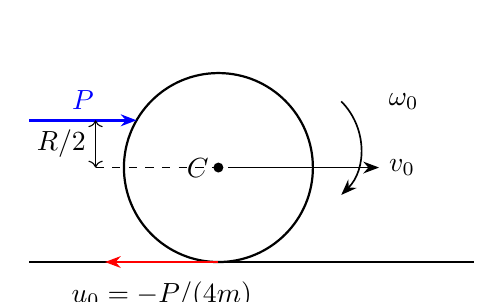
\begin{tikzpicture}[scale=1.2]
\draw[thick] (-2,0)--(2.7,0);
\draw[thick] (0,1) circle(1);
\fill (0,1) circle(1.5pt) node[left] {$C$};
\draw[arr,blue,very thick] (-2,1.5)--(-.866,1.5) node[midway,above] {$P$};
\draw[dashed] (-1.3,1)--(1,1);
\draw[<->] (-1.3,1)--(-1.3,1.5) node[midway,left] {$R/2$};
\draw[arr] (.2,1)--(1.7,1) node[right] {$v_0$};
\draw[arr] (1.3,1.7) arc(45:-45:.7);
\node[right] at (1.7,1.7) {$\omega_0$};
\draw[arr,red] (0,0)--(-1.2,0);
\node[below] at (-.6,-.1) {$u_0=-P/(4m)$};
\end{tikzpicture}
}
\ifdim\wd\diagrambox>.88\linewidth
\sbox{\diagrambox}{\resizebox{.88\linewidth}{!}{\usebox{\diagrambox}}}\fi
\ifdim\ht\diagrambox>.38\textheight
\resizebox{!}{.38\textheight}{\usebox{\diagrambox}}
\else\usebox{\diagrambox}\fi
\par\smallskip{\small 图2a　击打位置与初始接触点运动\par}\endgroup\end{minipage}\end{center}

（1）击打后经过多久母球开始纯滚动？求进入纯滚动时的球心速度。

（2）在开始纯滚动时将计时清零，记此时球上与桌面接触的材料点为\(B\)。求随后\(t'\)时刻\(B\)的位置、速度和加速度。

\subsection{一、题型定位}\label{ux4e00ux9898ux578bux5b9aux4f4d-1}

击打使球同时获得平动和转动；球底接触点是否滑动，要用这两种运动合成判断。本题的击打点较高，产生的自转使球底向后滑动，尽管球心向前运动。

在滑动阶段，摩擦朝前，加快球心同时减慢自转，直到\(v=R\omega\)。之后理想水平桌面不需要非零静摩擦维持匀速滚动。

第二问追踪的是固定材料点\(B\)，而非每个时刻不断更换的几何接触点。它随着球转动离开桌面，走过摆线；速度在触地点为零，加速度却仍非零。

\subsection{二、知识点}\label{ux4e8cux77e5ux8bc6ux70b9-1}

\subsubsection{1.
方向、惯量与冲量}\label{ux65b9ux5411ux60efux91cfux4e0eux51b2ux91cf}

取\(x\)水平向右，与球杆冲量同向；\(y\)竖直向上。用顺时针转动的角速度大小\(\omega\)作正标量。均质实心球绕球心的惯量为

\[
J=\frac25mR^2.
\]

击打前静止，极短击打中有限的桌面摩擦不能贡献可比于\(P\)的冲量。水平冲量和关于球心的角冲量分别给

\[
mv_0=P,\qquad J\omega_0=P\frac R2.
\]

因此击打后\(v_0=P/m\)，\(\omega_0=5P/(4mR)\)。两个结果来自不同守恒方程，不能先套纯滚动约束，因为此时尚在滑动。

\subsubsection{2.
接触点的有向速度}\label{ux63a5ux89e6ux70b9ux7684ux6709ux5411ux901fux5ea6}

球底相对球心的转动速度向左，故实际球底材料点相对桌面的水平速度

\[
u=v-R\omega.
\]

这个\(u\)决定滑动摩擦的方向：\(u<0\)时摩擦向右，\(u>0\)时摩擦向左。摩擦作用方向由局部相对滑动决定，不由质心运动方向决定。

\subsubsection{3.
刚体点的速度与加速度}\label{ux521aux4f53ux70b9ux7684ux901fux5ea6ux4e0eux52a0ux901fux5ea6}

对于球心\(C\)和固定材料点\(B\)，

\[
\mathbf v_B=\mathbf v_C+\boldsymbol\omega\times\mathbf r_{B/C},
\]

\[
\mathbf a_B=\mathbf a_C+
\dot{\boldsymbol\omega}\times\mathbf r_{B/C}
+\boldsymbol\omega\times
(\boldsymbol\omega\times\mathbf r_{B/C}).
\]

匀速纯滚动时\(\mathbf a_C=0\)、\(\dot{\boldsymbol\omega}=0\)，但最后的向心加速度存在。瞬时速度为零不能推出瞬时加速度为零。

\subsection{三、物理图像}\label{ux4e09ux7269ux7406ux56feux50cf-1}

击打线高于球心，关于球心的力矩为顺时针。代入\(v_0,\omega_0\)，

\[
u_0=\frac Pm-\frac{5P}{4m}
=-\frac P{4m}<0.
\]

因此球底向后擦桌面，桌面对球的摩擦向前。

\begin{center}
\begin{minipage}{\linewidth}
\centering\begingroup\sbox{\diagrambox}{\small
\begin{tikzpicture}[scale=1.15]
\draw[thick] (-1.8,0)--(2,0); \draw[thick] (0,1) circle(1);
\draw[arr,red,very thick] (0,0)--(1.3,0) node[right] {$f=\mu mg$};
\draw[arr] (0,1)--(0,.65); \node[left] at (-.1,.82) {$mg$};
\draw[arr] (0,0)--(0,.4); \node[right] at (.1,.2) {$N$};
\draw[arr,blue] (0,1)--(1.4,1) node[right] {$v$增大};
\node at (0,2.6) {$\omega$减小，$v-R\omega$趋零};
\end{tikzpicture}
}
\ifdim\wd\diagrambox>.88\linewidth
\sbox{\diagrambox}{\resizebox{.88\linewidth}{!}{\usebox{\diagrambox}}}\fi
\ifdim\ht\diagrambox>.38\textheight
\resizebox{!}{.38\textheight}{\usebox{\diagrambox}}
\else\usebox{\diagrambox}\fi
\par\smallskip{\small 图2b　滑动阶段的受力与速度\par}\endgroup\end{minipage}\end{center}

同一向右的摩擦对球心作顺时针反向力矩：它使\(v\)增大、\(\omega\)减小，所以\(v-R\omega\)从负值向零靠近。到达零后，平动和转动无须再交换动量。

纯滚动阶段，\(B\)从球底出发，先向右上方运动，到球顶时水平速度是球心速度的两倍，再回到下一个触地点。

\begin{center}
\begin{minipage}{\linewidth}
\centering\begingroup\sbox{\diagrambox}{\small
\begin{tikzpicture}[xscale=.9,yscale=.9]
\draw[arr] (-.4,0)--(7,0) node[right] {$x/R$};
\draw[arr] (0,0)--(0,2.7) node[above] {$y/R$};
\draw[dashed] (0,1)--(6.283,1);
\draw[thick,blue,domain=0:6.283,samples=140] plot({\x-sin(\x r)},{1-cos(\x r)});
\foreach \a in {0,3.1416,6.2832}{
\draw[gray] (\a,1) circle(1);
\fill[blue] ({\a-sin(\a r)},{1-cos(\a r)}) circle(2pt);}
\node[above] at (3.1416,2.1) {球顶：$v_B=2v_c$};
\node at (3.1,-.9) {$x_B/R=\theta-\sin\theta,\quad y_B/R=1-\cos\theta$};
\end{tikzpicture}
}
\ifdim\wd\diagrambox>.88\linewidth
\sbox{\diagrambox}{\resizebox{.88\linewidth}{!}{\usebox{\diagrambox}}}\fi
\ifdim\ht\diagrambox>.38\textheight
\resizebox{!}{.38\textheight}{\usebox{\diagrambox}}
\else\usebox{\diagrambox}\fi
\par\smallskip{\small 图2c　材料点B的摆线\par}\endgroup\end{minipage}\end{center}

图中的球心沿高度\(R\)的直线前进，材料点相对球心沿圆周顺时针转动。把这两个位移相加即可建立坐标参数式。

\subsection{四、解题入口}\label{ux56dbux89e3ux9898ux5165ux53e3-1}

分成击打、滑动、纯滚动三段。击打用线冲量与角冲量求初值；滑动先判断\(u_0\)，再写平动及转动方程；纯滚动之后重新计时，建立固定点的轨迹。

滑动终止条件只有一个：

\[
v(t_0)-R\omega(t_0)=0.
\]

它是过程边界，不是整个滑动阶段的恒等式。第二问用\(\theta=(v_c/R)t'\)作参数，能同时得到位置、速度和加速度。

\subsection{五、解析}\label{ux4e94ux89e3ux6790-1}

\subsubsection{（1）击打产生的初始运动}\label{ux51fbux6253ux4ea7ux751fux7684ux521dux59cbux8fd0ux52a8}

沿冲量方向应用动量定理，

\[
P=mv_0,\qquad \boxed{v_0=\frac Pm}.
\]

击打点到球心的垂直力臂为\(R/2\)，所以

\[
\frac{PR}{2}=J\omega_0
=\frac25mR^2\omega_0,
\]

得到

\[
\boxed{\omega_0=\frac{5P}{4mR}}.
\]

球底速度\(u_0=-P/(4m)\)，故摩擦恒朝正\(x\)，大小\(f=\mu mg\)，法向力与重力相消。

\subsubsection{滑动阶段的动力学}\label{ux6ed1ux52a8ux9636ux6bb5ux7684ux52a8ux529bux5b66}

平动方程

\[
m\dot v=\mu mg,
\qquad
v(t)=\frac Pm+\mu gt.
\]

取顺时针为正，球底向右的摩擦产生逆时针力矩，

\[
J\dot\omega=-\mu mgR.
\]

因此

\[
\dot\omega=-\frac{5\mu g}{2R},
\qquad
\omega(t)=\frac{5P}{4mR}-\frac{5\mu g}{2R}t.
\]

接触相对速度为

\[
\begin{aligned}
u(t)&=v(t)-R\omega(t)\\
&=-\frac P{4m}+\frac72\mu gt.
\end{aligned}
\]

在\(u<0\)的整个区间，所用摩擦方向一致。令\(u(t_0)=0\)，

\[
\boxed{t_0=\frac{P}{14\mu mg}}.
\]

这是从击打结束到第一次到达纯滚动条件的时间。\(\mu>0\)、\(P>0\)时\(t_0>0\)；若\(\mu=0\)，初始运动本来不满足滚动约束，因而永远不能靠桌面作用自行转成纯滚动。

\subsubsection{纯滚动初值}\label{ux7eafux6edaux52a8ux521dux503c}

代入\(t_0\)，

\[
v_c=\frac Pm+\frac P{14m}
=\boxed{\frac{15P}{14m}}.
\]

角速度为

\[
\omega_c=\frac{5P}{4mR}
-\frac{5P}{28mR}
=\frac{15P}{14mR}
=\frac{v_c}{R}.
\]

球心速度比击打刚结束时略大。桌面没有运动，摩擦仍耗散机械能；它可以增加平动动能，但同时减少更多转动动能。

\subsubsection{纯滚动之后为什么没有持续摩擦}\label{ux7eafux6edaux52a8ux4e4bux540eux4e3aux4ec0ux4e48ux6ca1ux6709ux6301ux7eedux6469ux64e6}

若此后仍假设向右静摩擦\(f_s\)，则

\[
m\dot v=f_s,\qquad J\dot\omega=-f_sR.
\]

纯滚动要求\(\dot v=R\dot\omega\)，所以

\[
\frac{f_s}{m}=-\frac{f_sR^2}{J},
\]

即\(f_s=0\)。原题不计滚动阻力，球以后保持\(v_c,\omega_c\)不变。最大静摩擦与滑动摩擦相等的条件允许过程平稳达到无滑动状态，但并不要求无滑动时静摩擦取最大值。

\subsubsection{角动量的独立检查}\label{ux89d2ux52a8ux91cfux7684ux72ecux7acbux68c0ux67e5}

在任意桌面固定点上方的运动中，取地面初始接触位置为矩心，桌面摩擦作用线过该地面水平线，力矩为零；重力与支持力的总力矩相消。等价地，在当前接触点处写可守恒的平动---自转组合，

\[
J\omega+mRv
=J\omega_0+mRv_0.
\]

由动力学直接求导也有

\[
J\dot\omega+mR\dot v
=-fR+fR=0.
\]

代入纯滚动\(\omega_c=v_c/R\)，

\[
\left(\frac JR+mR\right)v_c
=\frac{PR}{2}+PR,
\]

于是\(v_c=15P/(14m)\)。这条路线不用摩擦系数解释最终滚动速度，但不能仅凭它求滑动所需时间。

\subsubsection{耗散能量核对}\label{ux8017ux6563ux80fdux91cfux6838ux5bf9}

击打后动能

\[
K_0=\frac12mv_0^2+\frac12J\omega_0^2
=\frac{13P^2}{16m}.
\]

纯滚动动能

\[
K_c=\frac12\left(m+\frac J{R^2}\right)v_c^2
=\frac{45P^2}{56m}.
\]

差为

\[
\boxed{K_0-K_c=\frac{P^2}{112m}>0}.
\]

摩擦总功率是作用点速度与力的点积，

\[
\dot K=f[v-R\omega]=\mu mg\,u(t)<0.
\]

故

\[
\begin{aligned}
W_f&=\mu mg\int_0^{t_0}
\left(-\frac P{4m}+\frac72\mu gt\right)dt\\
&=-\frac{P^2}{112m},
\end{aligned}
\]

与动能差相符。只计算\(f\)乘球心位移会得到正功，遗漏了摩擦对自转的负功。

\subsubsection{（2）固定点B的位置}\label{ux56faux5b9aux70b9bux7684ux4f4dux7f6e}

在纯滚动开始时重置\(t'=0\)，以\(B\)当时接触桌面的点为坐标原点，球心初始位置\((0,R)\)。此后球心位置为

\[
(x_C,y_C)=(v_ct',R).
\]

令顺时针转角

\[
\theta=\omega_ct'=\frac{v_c}{R}t'.
\]

初始\(\mathbf r_{B/C}=(0,-R)\)，顺时针转\(\theta\)后，

\[
\mathbf r_{B/C}=(-R\sin\theta,-R\cos\theta).
\]

所以

\[
\boxed{
x_B=v_ct'-R\sin\theta
=R(\theta-\sin\theta)},
\]

\[
\boxed{y_B=R(1-\cos\theta)}.
\]

若需要全部用题给量表示，只需替换

\[
\theta=\frac{15Pt'}{14mR}.
\]

在\(\theta=0\)时\(B=(0,0)\)；\(\theta=\pi\)时\(B=(\pi R,2R)\)；\(\theta=2\pi\)时\(B=(2\pi R,0)\)，满足一圈前进\(2\pi R\)。

\subsubsection{速度及其分支}\label{ux901fux5ea6ux53caux5176ux5206ux652f}

位置对时间求导：

\[
\boxed{
\mathbf v_B=
v_c(1-\cos\theta)\,\hat{\mathbf x}
+v_c\sin\theta\,\hat{\mathbf y}}.
\]

速率由两分量的平方和给出，

\[
\begin{aligned}
|\mathbf v_B|
&=v_c\sqrt{(1-\cos\theta)^2+\sin^2\theta}\\
&=v_c\sqrt{2-2\cos\theta}\\
&=\boxed{2v_c\left|\sin\frac{\theta}{2}\right|}.
\end{aligned}
\]

对于\(0<\theta<2\pi\)，\(\sin(\theta/2)>0\)，可以去掉绝对值。若题目要求任意\(t'\)，必须保留绝对值，不能让第二圈速率变负。

速度方向最稳妥的完整表述是两个有向分量。第一圈非触地时，其与\(x\)轴的角度满足

\[
\alpha=\frac{\pi}{2}-\frac{\theta}{2},
\qquad 0<\theta<2\pi.
\]

角度在触地点速度为零时无定义。跨圈可用\(\operatorname{atan2}(\sin\theta,1-\cos\theta)\)，不把第一圈的单一线性角度公式无限延长。

\par\noindent\begin{minipage}{\linewidth}
\subsubsection{加速度}\label{ux52a0ux901fux5ea6}

再次求导，

\[
\boxed{
\mathbf a_B=
\frac{v_c^2}{R}\sin\theta\,\hat{\mathbf x}
+\frac{v_c^2}{R}\cos\theta\,\hat{\mathbf y}}.
\]

大小

\[
\boxed{
|\mathbf a_B|=\frac{v_c^2}{R}
=\frac{225P^2}{196m^2R}}.
\]

其方向始终指向球心，因为

\[
\mathbf a_B=-\omega_c^2\mathbf r_{B/C}.
\]

在\(t'=0\)，速度为零，加速度为\((0,v_c^2/R)\)；在球顶，加速度向下。球心匀速与材料点加速没有矛盾。

\subsubsection{触地点附近的轨迹检查}\label{ux89e6ux5730ux70b9ux9644ux8fd1ux7684ux8f68ux8ff9ux68c0ux67e5}

当\(\theta\)很小时，

\[
\sin\theta=\theta-\frac{\theta^3}{6}+O(\theta^5),
\quad
\cos\theta=1-\frac{\theta^2}{2}+O(\theta^4),
\]

故

\[
x_B=\frac R6\theta^3+O(\theta^5),
\quad
y_B=\frac R2\theta^2+O(\theta^4).
\]

水平速度从二次小量起步，竖直速度从一次小量起步，解释了摆线在触地点的尖点和竖直切向。尖点是轨迹几何性质，材料点的时间加速度依然有限。

\end{minipage}\par
\clearpage

\section{第 3
题　负微分电阻与RLC振荡（40分）}\label{ux7b2c-3-ux9898-ux8d1fux5faeux5206ux7535ux963bux4e0erlcux632fux836140ux5206}

某些电路或元件在特定电压范围内，电流随端电压增加而减小，称为负微分电阻效应。简化电路如图：左侧由电阻\(R\)、电感\(L\)、电容\(C\)和隧道二极管\(D\)形成交流回路，交流电流为\(i(t)\)；右侧由理想高频扼流圈RFC和理想直流电源\(V_0\)组成，直流电流为\(I\)，\(I\gg|i(t)|\)。RFC直流电阻为零，完全阻断交流。已标示电流方向。

\begin{center}
\begin{minipage}{\linewidth}
\centering\begingroup\sbox{\diagrambox}{\small
\begin{tikzpicture}[scale=.95]
\draw[thick] (0,0)--(0,.6); \draw[thick] (-.2,.6) rectangle(.2,1.4);
\node[left] at (-.2,1) {$R$}; \draw[thick] (0,1.4)--(0,2)--(.5,2);
\draw[thick,decorate,decoration={coil,aspect=.3,segment length=4pt,amplitude=3pt}] (.5,2)--(1.4,2);
\node[above] at (.95,2.25) {$L$};\draw[thick] (1.4,2)--(1.9,2);
\draw[thick] (1.9,1.7)--(1.9,2.3); \draw[thick] (2.1,1.7)--(2.1,2.3);
\node[above] at (2,2.3) {$C$}; \draw[thick] (2.1,2)--(3,2);
\draw[thick] (3,2)--(3,1.4); \draw[thick,fill=gray!12] (2.65,.6) rectangle(3.35,1.4);
\node at (3,1) {$D$};\draw[thick] (3,.6)--(3,0)--(0,0);
\node[right] at (3.4,1) {$r_d=-R_0$};
\draw[thick] (3,2)--(4,2);
\draw[thick,decorate,decoration={coil,aspect=.3,segment length=4pt,amplitude=3pt}] (4,2)--(5,2);
\node[above] at (4.5,2.3) {RFC};
\draw[thick] (5,2)--(6,2)--(6,1.4); \draw[thick] (6,1) circle(.4);
\node at (6,1) {$V_0$};\draw[thick] (6,.6)--(6,0)--(3,0);
\draw[arr,blue] (.7,1.3)--(1.8,1.3) node[midway,below] {$i(t)$};
\draw[arr,red] (5.7,3.1)--(3.4,3.1) node[midway,above] {$I$};
\node at (3,-.7) {左侧交流回路；右侧直流偏置};
\end{tikzpicture}
}
\ifdim\wd\diagrambox>.88\linewidth
\sbox{\diagrambox}{\resizebox{.88\linewidth}{!}{\usebox{\diagrambox}}}\fi
\ifdim\ht\diagrambox>.38\textheight
\resizebox{!}{.38\textheight}{\usebox{\diagrambox}}
\else\usebox{\diagrambox}\fi
\par\smallskip{\small 图3a　直流偏置与交流回路\par}\endgroup\end{minipage}\end{center}

二极管始终处于负微分电阻区，其微分电阻为\(-R_0\)，\(R_0>0\)且为常量。

（1）已知\(i(0)=0\)、\(\dot i(0)=\beta\neq0\)，且

\[
i(t)=\alpha_1e^{\beta_1t}+\alpha_2e^{\beta_2t},
\]

求各常数及任意时刻\(i(t)\)。

（2）求左侧产生持续等幅谐振的条件、电流\(i_H(t)\)和频率\(f_H\)。

（3）求左侧产生随时间衰减的RLC阻尼振荡的条件、电流\(i_D(t)\)及振荡频率\(f_D\)。

（4）二极管负微分电阻工作电压范围为\(V_{\min}\leq V_D\leq V_{\max}\)。求其交流部分能提供的最大平均功率\(\overline P_{\max}\)，以及此时直流电源电压\(V_0\)。

\subsection{一、题型定位}\label{ux4e00ux9898ux578bux5b9aux4f4d-2}

本题把非线性器件在一个工作点附近线性化，得到带负电阻的二阶自由响应。直流电源负责建立偏置并提供能量；交流回路的净耗散由\(R-R_0\)决定。

第一问求一般初值解，第二、三问从特征根的实部和虚部识别运动类型。第四问是有限工作区间内的正弦幅度与偏置优化，不是继续无限使用指数增长解。

初始电流导数非零意味着回路储能并非全为零。写积分形式的基尔霍夫方程时要保留电容初始电压，才能与初值兼容。

\subsection{二、知识点}\label{ux4e8cux77e5ux8bc6ux70b9-2}

\subsubsection{1.
直流和交流分解}\label{ux76f4ux6d41ux548cux4ea4ux6d41ux5206ux89e3}

将二极管电流与电压写作

\[
I_D=I+i,\qquad V_D=\overline V_D+v_d.
\]

负微分电阻定义是局部斜率

\[
v_d=-R_0i.
\]

这并非\(V_D=-R_0I_D\)；实际直流电压和电流都可以为正，整体器件仍从电源取能。\(-R_0\)描述交流扰动的电压---电流关系。

RFC让直流偏置通路可导通、交流扰动不能向右流。电容阻断左侧的直流，故直流电源电压等于二极管的平均端电压。

\subsubsection{2.
电容的初始常数}\label{ux7535ux5bb9ux7684ux521dux59cbux5e38ux6570}

按照交流回路电流方向取电容电压降\(v_C\)，

\[
\dot v_C=\frac{i}{C},
\qquad
v_C(t)=v_C(0)+\frac1C\int_0^ti(s)\,ds.
\]

交流KVL为

\[
L\dot i+(R-R_0)i+v_C=0.
\]

在\(t=0\)时\(i=0,\dot i=\beta\)，故

\[
\boxed{v_C(0)=-L\beta}.
\]

如果去掉\(v_C(0)\)，就会在\(t=0\)得到\(L\beta=0\)，与题设冲突。这个常数在微分后消失，但必须在初值解释和反代检查中保留。

\subsubsection{3.
二阶方程及特征根}\label{ux4e8cux9636ux65b9ux7a0bux53caux7279ux5f81ux6839}

将KVL对时间求导，

\[
L\ddot i+(R-R_0)\dot i+\frac iC=0.
\]

定义

\[
\delta=\frac{R-R_0}{2L},\qquad
\omega_0=\frac1{\sqrt{LC}}.
\]

方程变为

\[
\ddot i+2\delta\dot i+\omega_0^2i=0.
\]

若试解\(e^{st}\)，特征方程\(s^2+2\delta s+\omega_0^2=0\)，特征根

\[
s_\pm=-\delta\pm q,\qquad
q=\sqrt{\delta^2-\omega_0^2}.
\]

当判别式为负时\(q\)为纯虚数，最终电流仍是实函数；不能因为题目最初写指数形式就只允许实数根。

\subsubsection{4.
能量交换与净耗散}\label{ux80fdux91cfux4ea4ux6362ux4e0eux51c0ux8017ux6563}

回路瞬时储能

\[
U=\frac12Li^2+\frac12Cv_C^2.
\]

对时间求导并用KVL，

\[
\dot U=i(L\dot i+v_C)=-(R-R_0)i^2.
\]

电阻吸收\(Ri^2\)，二极管交流部分吸收\(-R_0i^2\)，其负值表示向交流回路输送能量。

\subsection{三、物理图像}\label{ux4e09ux7269ux7406ux56feux50cf-2}

\(R>R_0\)时二极管补充的交流能量小于电阻损耗，振幅衰减；\(R=R_0\)时两者恰好抵消；\(R<R_0\)时线性模型中的扰动增长。

\begin{center}
\begin{minipage}{\linewidth}
\centering\begingroup\sbox{\diagrambox}{\small
\begin{tikzpicture}[xscale=.5,yscale=1]
\draw[arr] (0,0)--(13.5,0) node[right] {$\omega_0t$};
\draw[arr] (0,-2)--(0,2.2) node[above] {$i/(\beta/\omega_0)$};
\begin{scope}\clip (0,-2) rectangle(13,2);
\foreach \d/\col in {.06/blue,0/black,-.06/red}{
\draw[thick,\col,domain=0:13,samples=180] plot(\x,{exp(-\d*\x)*sin(sqrt(1-\d*\d)*\x r)/sqrt(1-\d*\d)});}
\end{scope}
\node[blue] at (2,-2.6) {衰减};
\node at (6.5,-2.6) {等幅};
\node[red] at (11,-2.6) {增长};
\end{tikzpicture}
}
\ifdim\wd\diagrambox>.88\linewidth
\sbox{\diagrambox}{\resizebox{.88\linewidth}{!}{\usebox{\diagrambox}}}\fi
\ifdim\ht\diagrambox>.38\textheight
\resizebox{!}{.38\textheight}{\usebox{\diagrambox}}
\else\usebox{\diagrambox}\fi
\par\smallskip{\small 图3b　净阻尼改变时的电流响应\par}\endgroup\end{minipage}\end{center}

是否有振荡还需要特征根含虚部。正净阻尼既可能产生衰减振荡，也可能产生不振荡的过阻尼响应。

\begin{center}
\begin{minipage}{\linewidth}
\centering\begingroup\sbox{\diagrambox}{\small
\begin{tikzpicture}[xscale=2.8,yscale=1]
\draw[arr] (-1.6,0)--(1.7,0) node[right] {$\delta/\omega_0$};
\foreach \x in {-1,0,1}{\draw (\x,-.12)--(\x,.12); \node[below] at (\x,-.12) {$\x$};}
\draw[very thick,red] (-1,0)--(0,0);
\draw[very thick,blue] (0,0)--(1,0);
\node at (-1.3,1.1) {双实根增长};
\node[red] at (-.5,.6) {增长振荡};
\node[blue] at (.5,.6) {衰减振荡};
\node at (1.3,1.1) {双实根衰减};
\node at (0,-1) {$\delta=0$等幅；$\delta=\pm\omega_0$重根};
\end{tikzpicture}
}
\ifdim\wd\diagrambox>.88\linewidth
\sbox{\diagrambox}{\resizebox{.88\linewidth}{!}{\usebox{\diagrambox}}}\fi
\ifdim\ht\diagrambox>.38\textheight
\resizebox{!}{.38\textheight}{\usebox{\diagrambox}}
\else\usebox{\diagrambox}\fi
\par\smallskip{\small 图3c　特征根与振荡区间\par}\endgroup\end{minipage}\end{center}

图中横坐标\(\delta/\omega_0\)决定根的类型：\(|\delta|<\omega_0\)时有虚部；\(\delta>0\)时包络衰减；\(\delta=0\)时等幅；\(\delta<0\)时增长。二极管有限工作区间使增长最终离开本题线性模型，不能由常量负电阻预测稳定极限环。

\subsection{四、解题入口}\label{ux56dbux89e3ux9898ux5165ux53e3-2}

交流回路只保留左侧串联元件与二极管微分电阻。先写带初始电容电压的KVL，再微分得到二阶方程。

两根不等时用\(i(0)=0\)得到\(\alpha_2=-\alpha_1\)，再用\(\dot i(0)=\beta\)确定幅度。把指数差转成\(\sin\)或\(\sinh\)，可使各阻尼区间的实解更清楚。

第四问将电压写成偏置加正弦：平均值必须使正、负峰值都留在\([V_{\min},V_{\max}]\)内。峰值幅度与有效值不能混同，平均功率需要因子\(1/2\)。

\subsection{五、解析}\label{ux4e94ux89e3ux6790-2}

\subsubsection{（1）一般的非重根解}\label{ux4e00ux822cux7684ux975eux91cdux6839ux89e3}

特征根由\(Ls^2+(R-R_0)s+1/C=0\)给出，

\[
\boxed{
\beta_{1,2}
=-\frac{R-R_0}{2L}
\pm\sqrt{\left(\frac{R-R_0}{2L}\right)^2-\frac1{LC}}}.
\]

选择\(\beta_1=-\delta+q\)、\(\beta_2=-\delta-q\)。初值给

\[
\alpha_1+\alpha_2=0,
\qquad
\alpha_1\beta_1+\alpha_2\beta_2=\beta.
\]

因此\(q\neq0\)时

\[
\boxed{\alpha_1=\frac{\beta}{2q},\qquad
\alpha_2=-\frac{\beta}{2q}},
\]

并有

\[
\boxed{
i(t)=\frac{\beta}{2q}e^{-\delta t}
(e^{qt}-e^{-qt})
=\beta e^{-\delta t}\frac{\sinh(qt)}q}.
\]

根的编号可以交换，两个系数也随之交换，但电流不变。\(\beta\)是初始电流斜率，量纲A/s；\(\beta_1,\beta_2\)是特征增长率，量纲1/s。

\subsubsection{含初始电压的反代检查}\label{ux542bux521dux59cbux7535ux538bux7684ux53cdux4ee3ux68c0ux67e5}

由KVL定义

\[
v_C(t)=-L\dot i(t)-(R-R_0)i(t).
\]

该表达式在\(t=0\)给\(-L\beta\)。利用二阶方程求导，

\[
\dot v_C=-L\ddot i-(R-R_0)\dot i=\frac iC.
\]

于是它恰好满足

\[
v_C(t)=-L\beta+\frac1C\int_0^ti(s)\,ds.
\]

因此微分后得到的解确实可以恢复原始KVL，而非只满足一条丢失积分常数的方程。

\subsubsection{判别式负：实数振荡形式}\label{ux5224ux522bux5f0fux8d1fux5b9eux6570ux632fux8361ux5f62ux5f0f}

当\(|\delta|<\omega_0\)，定义

\[
\omega_d=\sqrt{\omega_0^2-\delta^2}>0,
\qquad q=i\omega_d.
\]

利用\(\sinh(ix)=i\sin x\)，一般解写为

\[
\boxed{
i(t)=\frac{\beta}{\omega_d}
e^{-\delta t}\sin(\omega_dt)}.
\]

初值验证：

\[
i(0)=0,\qquad
\dot i(0)=\frac{\beta}{\omega_d}\omega_d=\beta.
\]

振荡包络的增长或衰减由\(\delta\)符号决定；振荡的角频率则是\(\omega_d\)，不是包络指数。

\subsubsection{重根与临界边界}\label{ux91cdux6839ux4e0eux4e34ux754cux8fb9ux754c}

当\(\delta^2=\omega_0^2\)，原有``两不同指数''表示退化。正确基解为\(e^{-\delta t}\)和\(te^{-\delta t}\)，初值给

\[
\boxed{i(t)=\beta t\,e^{-\delta t}}.
\]

也可取\(q\to0\)：

\[
\lim_{q\to0}\frac{\sinh(qt)}q=t.
\]

对于\(\delta=+\omega_0\)，它是临界阻尼衰减；对于\(\delta=-\omega_0\)，它是临界边界的增长解。不能将分母\(q=0\)解释为电流无穷大，分子同时趋零。

\subsubsection{判别式正：不振荡的双指数}\label{ux5224ux522bux5f0fux6b63ux4e0dux632fux8361ux7684ux53ccux6307ux6570}

当\(\delta^2>\omega_0^2\)，\(q\)为实正数，电流仍使用\(\sinh\)表达式。若\(\delta>\omega_0\)，\(-\delta\pm q\)都为负，电流先从零上升再衰减，不周期过零。

若\(\delta<-\omega_0\)，两个特征根都为正，扰动不振荡地增长。虽然二极管供能，这并不自动构成正弦自激振荡。

\subsubsection{（2）持续等幅谐振}\label{ux6301ux7eedux7b49ux5e45ux8c10ux632f}

等幅非零响应要求能量不随时间减小或增加，因此

\[
R-R_0=0.
\]

此时\(\delta=0\)，自动满足\(\delta^2<\omega_0^2\)。有

\[
\boxed{R=R_0},
\]

\[
\boxed{
i_H(t)=\beta\sqrt{LC}\,
\sin\left(\frac t{\sqrt{LC}}\right)},
\]

\[
\boxed{f_H=\frac1{2\pi\sqrt{LC}}}.
\]

LC在电场能与磁场能之间往返交换，普通电阻的每周期损失由二极管从直流偏置供给的能量补偿。在这个理想常量斜率模型中，没有任何机制选择唯一的稳定振幅。

若初始\(\beta=0\)且\(i(0)=0\)，方程的零解将永久保持零；负电阻不会凭空制造确定初始扰动。题给\(\beta\neq0\)提供了启动响应。

\subsubsection{（3）衰减振荡的两个条件}\label{ux8870ux51cfux632fux8361ux7684ux4e24ux4e2aux6761ux4ef6}

衰减需要\(\delta>0\)；有振荡需要\(\delta^2<\omega_0^2\)。合并得到

\[
0<R-R_0<2\sqrt{\frac LC},
\]

即

\[
\boxed{R_0<R<R_0+2\sqrt{\frac LC}}.
\]

这不是所有``阻尼''响应的范围，只是欠阻尼振荡的范围。上边界为重根，超过它仍能衰减，但不振荡。

电流为

\[
\boxed{
i_D(t)=\frac{\beta}{\omega_d}
\exp\left[-\frac{R-R_0}{2L}t\right]
\sin(\omega_dt)},
\]

其中

\[
\omega_d=
\sqrt{\frac1{LC}-\left(\frac{R-R_0}{2L}\right)^2}.
\]

振荡频率

\[
\boxed{
f_D=\frac1{2\pi}
\sqrt{\frac1{LC}-\left(\frac{R-R_0}{2L}\right)^2}}.
\]

因为\(\omega_d<\omega_0\)，阻尼振荡频率比无阻尼频率小。相邻同向峰值的时间间隔为\(2\pi/\omega_d\)，包络每周期下降因子为\(e^{-2\pi\delta/\omega_d}\)。

\subsubsection{能量随时间的闭合}\label{ux80fdux91cfux968fux65f6ux95f4ux7684ux95edux5408}

初始\(i(0)=0\)，全部交流储能在电容中：

\[
U_0=\frac12CL^2\beta^2.
\]

当\(R>R_0\)且响应衰减到零，

\[
\int_0^\infty(R-R_0)i^2\,dt=U_0.
\]

不是只有电阻\(R\)耗尽这份初始能量；二极管在衰减过程中仍向交流回路补充\(R_0\int i^2dt\)，故普通电阻吸收的总能量更大。

对于欠阻尼解，可以显式积分验证：

\[
\int_0^\infty i^2dt
=\frac{\beta^2}{\omega_d^2}
\int_0^\infty e^{-2\delta t}\sin^2(\omega_dt)\,dt.
\]

利用\(\sin^2x=(1-\cos2x)/2\)，

\[
\int_0^\infty e^{-2\delta t}\sin^2(\omega_dt)\,dt
=\frac{\omega_d^2}{4\delta(\delta^2+\omega_d^2)}.
\]

因此

\[
\int_0^\infty i^2dt=\frac{\beta^2}{4\delta\omega_0^2}.
\]

乘\(R-R_0=2L\delta\)得\(CL^2\beta^2/2\)，与初始电容能一致。

\subsubsection{（4）偏置电压与允许正弦幅度}\label{ux504fux7f6eux7535ux538bux4e0eux5141ux8bb8ux6b63ux5f26ux5e45ux5ea6}

设二极管上的交流电压是

\[
v_d(t)=V_a\cos(\omega t+\varphi),
\qquad V_a\geq0.
\]

保持整个周期在负电阻区要求

\[
V_a\leq\overline V_D-V_{\min},
\qquad
V_a\leq V_{\max}-\overline V_D.
\]

两边余量的较小值决定最大幅度。为使它最大，偏置应位于区间中点：

\[
\boxed{
\overline V_D=\frac{V_{\max}+V_{\min}}2},
\]

\[
\boxed{V_{a,\max}=\frac{V_{\max}-V_{\min}}2}.
\]

\begin{center}
\begin{minipage}{\linewidth}
\centering\begingroup\sbox{\diagrambox}{\small
\begin{tikzpicture}[xscale=1,yscale=2.4]
\draw[arr] (0,0)--(6.8,0) node[right] {$\omega t$};
\draw[arr] (0,0)--(0,1.25) node[above] {$V_D$};
\draw[dashed] (0,1)--(6.3,1) node[right] {$V_{\max}$};
\draw[dashed] (0,.5)--(6.3,.5) node[right] {中点};
\node[left] at (0,0) {$V_{\min}$};
\draw[thick,blue,domain=0:6.283,samples=100] plot(\x,{.5+.5*sin(\x r)});
\draw[thick,red,domain=0:6.283,samples=100] plot(\x,{.75+.25*sin(\x r)});
\node[blue] at (2,-.3) {中点：最大幅度};
\node[red] at (5,-.6) {偏置偏移：幅度减少};
\end{tikzpicture}
}
\ifdim\wd\diagrambox>.88\linewidth
\sbox{\diagrambox}{\resizebox{.88\linewidth}{!}{\usebox{\diagrambox}}}\fi
\ifdim\ht\diagrambox>.38\textheight
\resizebox{!}{.38\textheight}{\usebox{\diagrambox}}
\else\usebox{\diagrambox}\fi
\par\smallskip{\small 图3d　直流偏置与交流电压的工作区间\par}\endgroup\end{minipage}\end{center}

图中上下峰值分别接触区间端点。偏置向任一端移动都会缩小可容纳的完整正弦幅度。

\subsubsection{最大交流输出功率}\label{ux6700ux5927ux4ea4ux6d41ux8f93ux51faux529fux7387}

由\(v_d=-R_0i\)，二极管交流吸收功率

\[
p_{\rm abs}=v_di=-\frac{v_d^2}{R_0}.
\]

对正弦取平均，

\[
\overline P_{\rm abs}=-\frac{V_a^2}{2R_0}.
\]

它提供给交流回路的功率大小为相反数，故

\[
\boxed{
\overline P_{\max}
=\frac{(V_{\max}-V_{\min})^2}{8R_0}}.
\]

这是题目与参考解答所求的最大正弦交流输出功率。若另允许方波等非正弦信号，平均平方值和谐波电路都改变，不能沿用同一\(1/2\)因子。

RFC的直流压降为零，理想直流电源与二极管构成直流回路，所以

\[
\boxed{V_0=\overline V_D
=\frac{V_{\max}+V_{\min}}2}.
\]

若还要求\(R=R_0\)的等幅响应达到这个幅度，由\(i_H\)的幅值\(|\beta|\sqrt{LC}\)可知

\[
R_0|\beta|\sqrt{LC}
=\frac{V_{\max}-V_{\min}}2.
\]

第四问的幅度优化不自动更改第一问指定的初值；它表示在允许工作区间内可实现的最大正弦响应。

\subsubsection{模型边界检查}\label{ux6a21ux578bux8fb9ux754cux68c0ux67e5}

微分电阻是常量的区间有限。若\(R<R_0\)，指数包络最终离开区间；之后必须使用二极管的真实非线性特性才能讨论饱和、削顶或稳定振幅。

原题\(V_{\min},V_{\max}\)只给电压范围，不能据此推导完整的非线性电流曲线。本题可以判断线性响应何时不再适用，却不能把无限增长当成器件真实输出。

\clearpage

\section{第 4
题　同步加速器磁场与反质子产生阈值（40分）}\label{ux7b2c-4-ux9898-ux540cux6b65ux52a0ux901fux5668ux78c1ux573aux4e0eux53cdux8d28ux5b50ux4ea7ux751fux9608ux503c40ux5206}

回旋加速器利用两个半圆形磁场使带电粒子沿圆弧转向，粒子反复经过两半圆缝隙间的高频电场而获得能量。某同步质子加速器Tevatron的粒子运行最大圆形轨道周长为\(L_{\max}=6436\)
m，可将质子加速到最大能量\(E_{p,\max}=1.00\times10^6\) MeV。

（1）粒子始终在垂直于均匀磁场的平面内运动，不计辐射损失。求达到该最大能量所需要的最小磁感应强度\(B_{\min}\)。

\begin{center}
\begin{minipage}{\linewidth}
\centering\begingroup\sbox{\diagrambox}{\small
\begin{tikzpicture}[scale=1]
\draw[thick] (0,0) circle(2);
\draw[arr] (2,0) arc(0:65:2);
\draw[arr] (0,2)--(-1.4,2) node[left] {$\mathbf p$};
\draw[arr,red] (0,2)--(0,.7) node[left] {$e\mathbf v\times\mathbf B$};
\draw[arr] (0,0)--(2,0) node[midway,below] {$R$};
\foreach \x/\y in {-1/-1,1/1,1/-1}{\node at (\x,\y) {$\otimes$};}
\node at (0,-2.8) {$p=eBR,\quad 2\pi R\leq L_{\max}$};
\node at (3.1,.7) {$\mathbf B$入纸面};
\end{tikzpicture}
}
\ifdim\wd\diagrambox>.88\linewidth
\sbox{\diagrambox}{\resizebox{.88\linewidth}{!}{\usebox{\diagrambox}}}\fi
\ifdim\ht\diagrambox>.38\textheight
\resizebox{!}{.38\textheight}{\usebox{\diagrambox}}
\else\usebox{\diagrambox}\fi
\par\smallskip{\small 图4a　磁场弯转与轨道周长限制\par}\endgroup\end{minipage}\end{center}

（2）高能质子撞击静止质子，可产生反质子，反应为

\[
p+p\longrightarrow p+p+p+\overline p.
\]

求入射质子产生反质子的最小动能，并判断上述加速器能否实现此反应。

已知\(m_pc^2=938.3\) MeV，\(c=3.00\times10^8\)
m/s。第一问给定能量按质子总能量使用。

\subsection{一、题型定位}\label{ux4e00ux9898ux578bux5b9aux4f4d-3}

第一问是相对论动量与磁场弯转半径的关系，第二问是固定靶反应的能量---动量阈值。两个问题都不能仅用牛顿动能\(mv^2/2\)。

磁场提供转向力而不做功；电场才使粒子获得能量。所求磁场是让已有高能质子留在允许圆轨道内的弯转场。

产生新粒子不只需要静能：固定靶入射体系有净动量，即使在阈值，末态在实验室里仍整体运动。因此阈值动能比新增的一对质子与反质子的静能\(2m_pc^2\)大。

\subsection{二、知识点}\label{ux4e8cux77e5ux8bc6ux70b9-3}

\subsubsection{1.
相对论动量与能量}\label{ux76f8ux5bf9ux8bbaux52a8ux91cfux4e0eux80fdux91cf}

质子总能量与动量为

\[
E=\gamma m_pc^2,\quad
p=\gamma m_pv,\quad
\gamma=\frac1{\sqrt{1-v^2/c^2}}.
\]

两者满足

\[
E^2=p^2c^2+m_p^2c^4,
\]

所以

\[
pc=\sqrt{E^2-m_p^2c^4}.
\]

总能量\(E\)包含静能，动能\(K=E-m_pc^2\)。同一反应中必须保持这一区分。

\subsubsection{2.
磁场中的弯转}\label{ux78c1ux573aux4e2dux7684ux5f2fux8f6c}

洛伦兹方程是动量的变化率：

\[
\frac{d\mathbf p}{dt}
=e\,\mathbf v\times\mathbf B.
\]

磁力与速度垂直，因而不改变\(E\)和\(p\)的大小，只改变动量方向。圆轨道上动量每单位时间转过角度\(v/R\)，故

\[
\left|\frac{d\mathbf p}{dt}\right|
=p\frac vR.
\]

与磁力大小\(evB\)比较，

\[
\boxed{p=eBR}.
\]

这个式子对相对论与非相对论圆轨道都适用，因为它直接使用动量，不把\(dp/dt\)错写为常质量\(m_p\,dv/dt\)。

\subsubsection{3. 体系不变量}\label{ux4f53ux7cfbux4e0dux53d8ux91cf}

把总能量和总动量组成四动量，能量平方形式的不变量为

\[
\mathcal S=E_{\rm tot}^2-c^2|\mathbf p_{\rm tot}|^2.
\]

它在各惯性系相同。质心系总动量为零，所以\(\sqrt{\mathcal S}\)就是该系可用的总能量。

四个末态粒子质量均为\(m_p\)，在质心系至少有静能\(4m_pc^2\)，阈值时各粒子相对质心都静止：

\[
\sqrt{\mathcal S_{\rm th}}=4m_pc^2.
\]

这不表示它们在实验室静止。实验室原先有入射动量，末态整体必须继续携带它。

\subsection{三、物理图像}\label{ux4e09ux7269ux7406ux56feux50cf-3}

在相同动量下，轨道半径越大，所需弯转场越小。允许周长上限意味着半径上限，最小磁场在最大半径处实现。

第二问中，实验室的靶质子静止，而质心系中两个入射质子相向运动。阈值末态在质心系聚为共同零动量状态，回到实验室后一起运动。

\begin{center}
\begin{minipage}{\linewidth}
\centering\begingroup\sbox{\diagrambox}{\small
\begin{tikzpicture}[scale=1]
\node at (-.3,2.9) {固定靶初态};
\fill[blue] (0,1.8) circle(3pt); \draw[arr,blue] (0,1.8)--(1.5,1.8);
\node[above] at (.6,1.9) {$E_1,p_1$};
\fill (3,1.8) circle(3pt); \node[above] at (3,2) {靶静止};
\node at (-.3,.4) {阈值末态};
\foreach \x/\lab in {0/p,.8/p,1.6/p,2.4/\bar p}{
\fill[red] (\x,-.3) circle(3pt); \node[below] at (\x,-.4) {$\lab$};
\draw[arr,red] (\x,-.3)--(\x+.45,-.3);}
\node at (2,-1.3) {实验室同速；质心系各自静止};
\end{tikzpicture}
}
\ifdim\wd\diagrambox>.88\linewidth
\sbox{\diagrambox}{\resizebox{.88\linewidth}{!}{\usebox{\diagrambox}}}\fi
\ifdim\ht\diagrambox>.38\textheight
\resizebox{!}{.38\textheight}{\usebox{\diagrambox}}
\else\usebox{\diagrambox}\fi
\par\smallskip{\small 图4b　固定靶与质心系阈值\par}\endgroup\end{minipage}\end{center}

图中的末态实验室速度相同，表示没有相对动能可再减少。它们仍具有整体动能，这是固定靶阈值升高的原因。

\subsection{四、解题入口}\label{ux56dbux89e3ux9898ux5165ux53e3-3}

先由给定总能量算\(pc\)，再由\(p=eBR\)和\(2\pi R\leq L_{\max}\)求\(B_{\min}\)。

第二问在实验室写总能量\(E_1+m_pc^2\)与总动量\(p_1\)，计算不变量：

\[
\mathcal S=(E_1+m_pc^2)^2-p_1^2c^2.
\]

用单个入射质子的\(E_1^2-p_1^2c^2=m_p^2c^4\)消元，再与阈值\((4m_pc^2)^2\)比较，最后从总能量减去静能得到动能。

\subsection{五、解析}\label{ux4e94ux89e3ux6790-3}

\subsubsection{（1）最大轨道与最小磁场}\label{ux6700ux5927ux8f68ux9053ux4e0eux6700ux5c0fux78c1ux573a}

圆轨道周长不得超过\(L_{\max}\)：

\[
2\pi R\leq L_{\max},\qquad
R\leq R_{\max}=\frac{L_{\max}}{2\pi}.
\]

固定\(p\)时\(B=p/(eR)\)，因此

\[
B\geq\frac p{eR_{\max}}
=\frac{2\pi p}{eL_{\max}}.
\]

不等号方向须保持一致：半径有上限，磁场有下限。达到下限时轨道恰好占满最大允许周长。

由能量---动量关系，

\[
\boxed{
B_{\min}=
\frac{2\pi}{ecL_{\max}}
\sqrt{E_{p,\max}^2-m_p^2c^4}}.
\]

这是精确的相对论表达式。高能近似\(E\gg m_pc^2\)时可用\(p\simeq E/c\)，但不应在阈值低能计算里直接使用该近似。

\subsubsection{能量单位转换}\label{ux80fdux91cfux5355ux4f4dux8f6cux6362}

题给能量用MeV。对单个单位电荷的质子，\(1\) eV\(/e=1\)
V，所以在\(\sqrt{E^2-m_p^2c^4}/e\)中可以将MeV数值乘\(10^6\)，直接得到伏特单位：

\[
\frac1e\sqrt{E^2-m_p^2c^4}
=10^6\sqrt{(10^6)^2-(938.3)^2}\ \mathrm V.
\]

故

\[
B_{\min}
=\frac{2\pi\times10^6}
{(3.00\times10^8)(6436)}
\sqrt{(10^6)^2-(938.3)^2}\ \mathrm T
\simeq\boxed{3.25\ \mathrm T}.
\]

参考解答给约3.26 T；按题给\(c,L_{\max}\)保留中间值计算为3.25
T，两者相差约0.2\%，属于同一约3.3 T的量级。

轨道半径约\(1.02\times10^3\) m。对于\(E=10^6\)
MeV，\(\gamma=E/(m_pc^2)\simeq1066\)，速度非常接近\(c\)；动量仍可随能量显著增加，不能因速度接近\(c\)就认为磁场不再需要增加。

\subsubsection{相对论高能近似误差}\label{ux76f8ux5bf9ux8bbaux9ad8ux80fdux8fd1ux4f3cux8befux5dee}

令\(\epsilon=m_pc^2/E\)，则

\[
pc=E\sqrt{1-\epsilon^2}
=E\left(1-\frac{\epsilon^2}{2}+O(\epsilon^4)\right).
\]

本题\(\epsilon\simeq9.38\times10^{-4}\)，忽略静能平方产生的相对误差约\(4.4\times10^{-7}\)，远小于题给常数的有效数字误差。该误差估计说明近似\(p\simeq E/c\)在第一问的精度要求内可用。

\subsubsection{弯转角的另一条推导}\label{ux5f2fux8f6cux89d2ux7684ux53e6ux4e00ux6761ux63a8ux5bfc}

在圆轨道上经过微小弧长\(ds\)时，动量方向变化\(d\theta=ds/R\)。磁力提供动量变化

\[
dp_\perp=evB\,dt=eB\,ds.
\]

又有\(dp_\perp=p\,d\theta=p\,ds/R\)，所以\(p=eBR\)。此推导直接使用弧长和动量方向变化，也避免相对论加速度公式的混淆。

磁场对每个微元所作功仍为

\[
dW=e(\mathbf v\times\mathbf B)\cdot\mathbf v\,dt=0.
\]

因此``达到某能量所需磁场''在此意为容纳该能量的圆轨道弯转磁场；粒子的能量增长由装置中的电场完成。

\subsubsection{（2）固定靶初态不变量}\label{ux56faux5b9aux9776ux521dux6001ux4e0dux53d8ux91cf}

记入射质子总能量为\(E_1\)、动量为\(p_1\)。靶质子静止，能量\(m_pc^2\)，动量零。实验室总量为

\[
E_{\rm tot}=E_1+m_pc^2,\qquad
p_{\rm tot}=p_1.
\]

所以

\[
\begin{aligned}
\mathcal S
&=(E_1+m_pc^2)^2-p_1^2c^2\\
&=(E_1^2-p_1^2c^2)+2E_1m_pc^2+m_p^2c^4\\
&=2m_p^2c^4+2E_1m_pc^2.
\end{aligned}
\]

每个末态粒子在质心系的能量都不小于其静能，故

\[
\sqrt{\mathcal S}\geq4m_pc^2.
\]

阈值取等号，

\[
2m_p^2c^4+2E_{1,\rm th}m_pc^2
=16m_p^2c^4.
\]

解得

\[
\boxed{E_{1,\rm th}=7m_pc^2}.
\]

题目要的是最小动能：

\[
\boxed{
K_{1,\rm th}=E_{1,\rm th}-m_pc^2
=6m_pc^2=5629.8\ \mathrm{MeV}}.
\]

相应最小总能量\(7(938.3)=6568.1\) MeV。不能把6568.1
MeV直接标成动能，也不能只按多出来的一对粒子写1876.6 MeV。

\subsubsection{实验室末态的共同运动}\label{ux5b9eux9a8cux5ba4ux672bux6001ux7684ux5171ux540cux8fd0ux52a8}

阈值初态入射动量

\[
p_{1,\rm th}c=
\sqrt{(7m_pc^2)^2-(m_pc^2)^2}
=4\sqrt3\,m_pc^2.
\]

质心系相对于实验室的速度为

\[
V_{\rm cm}=\frac{c^2p_{\rm tot}}{E_{\rm tot}}
=\frac{4\sqrt3}{8}c
=\frac{\sqrt3}{2}c,
\]

洛伦兹因子

\[
\gamma_{\rm cm}=2.
\]

阈值时四个末态粒子在质心系静止，因此在实验室各自总能量\(2m_pc^2\)、动量大小\(\sqrt3m_pc\)且方向相同。相加得到

\[
E_{\rm final}=8m_pc^2,\qquad
p_{\rm final}=4\sqrt3m_pc,
\]

与入射质子加静止靶质子的总量完全一致。这是对阈值条件的具体运动学核对。

\subsubsection{为何共同速度使总能量最小}\label{ux4e3aux4f55ux5171ux540cux901fux5ea6ux4f7fux603bux80fdux91cfux6700ux5c0f}

在固定总动量下，末态若存在相对运动，质心系还有正动能。把这种相对运动减到零，质心系总能量降到四个静能之和，同时保留实验室所需的整体动量。

可以将四个粒子视为共同速度的总静质量\(4m_p\)系统，其实验室总能量最小为

\[
E_{\rm final,min}
=\sqrt{(4m_pc^2)^2+p_1^2c^2}.
\]

能量守恒要求

\[
E_1+m_pc^2
\geq\sqrt{16m_p^2c^4+p_1^2c^2}.
\]

两边平方并消去\(p_1\)，同样得到\(E_1\geq7m_pc^2\)。这条路线不用先命名不变量，其依据仍是能量和动量同时守恒。

\par\noindent\begin{minipage}{\linewidth}
\subsubsection{加速器是否能产生反质子}\label{ux52a0ux901fux5668ux662fux5426ux80fdux4ea7ux751fux53cdux8d28ux5b50}

比较总能量：

\[
1.00\times10^6\ \mathrm{MeV}
>6568.1\ \mathrm{MeV}.
\]

因此题设最大能量远超过固定靶产生反质子的运动学阈值，结论为可以。该判断只说明反应在能量---动量守恒上允许，不从阈值推断实际反应概率或产额。

电荷与重子数也一致：初态电荷\(+2e\)，末态三个质子与一个反质子合计\(+2e\)；初态重子数2，末态\(3-1=2\)。阈值计算与这些守恒条件共同定义题给反应。

\end{minipage}\par
\clearpage

\section{第 5
题　飞行器间光信号与相对论投递（40分）}\label{ux7b2c-5-ux9898-ux98deux884cux5668ux95f4ux5149ux4fe1ux53f7ux4e0eux76f8ux5bf9ux8bbaux6295ux901240ux5206}

在惯性系\(\Sigma\)的\(Oxy\)坐标中，飞行器甲、乙沿同一条直线朝\(-y\)匀速飞行，丙在与之平行、相距\(d\)的另一条直线上朝\(+y\)匀速飞行。速度为

\[
\mathbf v_{\text{甲}\Sigma}=-\frac{2c}{3}\hat{\mathbf y},
\quad
\mathbf v_{\text{乙}\Sigma}=-\frac c3\hat{\mathbf y},
\quad
\mathbf v_{\text{丙}\Sigma}=\frac{2c}{3}\hat{\mathbf y}.
\]

甲、乙所在直线为\(x=0\)，丙所在直线为\(x=d\)；原图乙在甲的\(-y\)一侧。飞行器尺寸远小于\(d\)。

\begin{center}
\begin{minipage}{\linewidth}
\centering\begingroup\sbox{\diagrambox}{\small
\begin{tikzpicture}[scale=1]
\draw[arr] (-.5,0)--(5,0) node[right] {$x$};
\draw[arr] (0,0)--(0,4.2) node[above] {$y$};
\node[left] at (0,3.4) {甲};\draw[arr,blue] (0,3.4)--(0,2.5);
\node[left] at (0,1.4) {乙};\draw[arr] (0,1.4)--(0,.6);
\draw[dashed] (3.7,0)--(3.7,4);
\node[right] at (3.7,1.4) {丙};\draw[arr,red] (3.7,1.4)--(3.7,2.4);
\draw[<->] (0,-.6)--(3.7,-.6) node[midway,below] {$d$};
\node at (1.8,5.2) {$v_\text{甲}=-2c/3,\ v_\text{乙}=-c/3,\ v_\text{丙}=2c/3$};
\end{tikzpicture}
}
\ifdim\wd\diagrambox>.88\linewidth
\sbox{\diagrambox}{\resizebox{.88\linewidth}{!}{\usebox{\diagrambox}}}\fi
\ifdim\ht\diagrambox>.38\textheight
\resizebox{!}{.38\textheight}{\usebox{\diagrambox}}
\else\usebox{\diagrambox}\fi
\par\smallskip{\small 图5a　三艘飞行器的航线\par}\endgroup\end{minipage}\end{center}

（1）甲向乙发射光信号，乙收到后立即反射回甲。甲上原子钟测得从发射到收到返回光的时间为\(T\)。求\(\Sigma\)中和乙上观察者测得的这两事件的时间间隔；再求在甲系中，从甲收到返回光到甲追上乙的时间。

（2）甲与丙在\(\Sigma\)中相距最近时，甲发射质量和尺寸均可忽略的小货物。货物在\(\Sigma\)中的速率为\(3c/4\)，要求丙恰好收到它。求甲系中货物发射速度的大小及方向，并求乙系中货物从甲发射到丙接收的时间间隔。

\subsection{一、题型定位}\label{ux4e00ux9898ux578bux5b9aux4f4d-4}

本题同时涉及固有时、异地事件的时间变换和二维速度变换。第一问光信号的发射与返回都发生在甲上，所以\(T\)是甲的固有时；第二问货物的发射与接收发生在不同飞行器，不能直接套同一时间膨胀公式。

选择最容易描述的参考系来写事件，再把完整的时间和位置差转换到目标系。光信号问题在甲系中图像清楚，货物拦截问题在\(\Sigma\)中几何最简单。

方向答案应说明相对于哪条轴或哪艘飞行器的运动方向。只写一个角度而不说明参考方向，会把接近正\(y\)与接近负\(y\)的两个角混淆。

\subsection{二、知识点}\label{ux4e8cux77e5ux8bc6ux70b9-4}

\subsubsection{1.
沿y方向的洛伦兹变换}\label{ux6cbfyux65b9ux5411ux7684ux6d1bux4f26ux5179ux53d8ux6362}

设\(\Sigma'\)相对于\(\Sigma\)以速度\(v\hat{\mathbf y}\)运动，则

\[
t'=\gamma_v\left(t-\frac{vy}{c^2}\right),
\quad
y'=\gamma_v(y-vt),
\quad x'=x,
\]

其中\(\gamma_v=(1-v^2/c^2)^{-1/2}\)。对任意两个事件，

\[
\Delta t'=\gamma_v
\left(\Delta t-\frac{v\Delta y}{c^2}\right).
\]

当\(v\)为负时，仍代入有向值，不应把式中\(v\)先换成速率再凭直觉补符号。

\subsubsection{2.
固有时的条件}\label{ux56faux6709ux65f6ux7684ux6761ux4ef6}

如果两个事件在\(\Sigma'\)的同一位置，\(\Delta y'=0\)，该位置的钟直接测得固有时\(\Delta\tau=\Delta t'\)，并有\(\Delta t=\gamma_v\Delta\tau\)。

发射与收到返回光同在甲上，故可用时间膨胀求\(\Sigma\)间隔。乙观察这两事件的间隔一般是其坐标时间，不是某一只乙钟在两事件处的读数差。

\subsubsection{3.
一维与二维速度变换}\label{ux4e00ux7ef4ux4e0eux4e8cux7ef4ux901fux5ea6ux53d8ux6362}

对沿\(y\)的系间变换，

\[
u'_y=\frac{u_y-v}{1-vu_y/c^2},
\qquad
u'_x=\frac{u_x}
{\gamma_v(1-vu_y/c^2)}.
\]

垂直分量也会改变，因为时间坐标改变。只对纵向分量作相对论加法、横向分量保持原值，是错误的二维速度变换。

\subsubsection{4.
最近位置与拦截条件}\label{ux6700ux8fd1ux4f4dux7f6eux4e0eux62e6ux622aux6761ux4ef6}

平行航线的横向距离固定为\(d\)。甲与丙在\(\Sigma\)中最近时，其\(y\)坐标相同。可将这一时刻和甲的位置选为\(t=0\)、原点，不改变题目事件的时间间隔。

若货物从甲此时出发，丙没有\(x\)运动，恰好接收要求货物\(x\)位移等于\(d\)，同时货物和丙的\(y\)位移相同。

\subsection{三、物理图像}\label{ux4e09ux7269ux7406ux56feux50cf-4}

在\(\Sigma\)中，甲向负\(y\)运动比乙快；由于乙起初在前方的负\(y\)一侧，甲将逐渐追上乙。光先向负\(y\)追到乙，再向正\(y\)返回甲。

\begin{center}
\begin{minipage}{\linewidth}
\centering\begingroup\sbox{\diagrambox}{\small
\begin{tikzpicture}[xscale=3.5,yscale=3.5]
\draw[arr] (-1.3,0)--(.3,0) node[right] {$y/(cT)$};
\draw[arr] (0,0)--(0,1.6) node[above] {$t/T$};
\draw[dashed,thick] (0,0)--(-.98,1.47);
\draw[dashed,thick] (-.74536,0)--(-1.23536,1.47);
\draw[arr,blue,thick] (0,0)--(-1.118034,1.118034);
\draw[arr,blue,thick] (-1.118034,1.118034)--(-.894427,1.341641);
\node[below right] at (0,0) {$A$};
\node[left] at (-1.118034,1.118034) {$B$反射};
\node[above right] at (-.894427,1.341641) {$C$返回};
\node at (-.65,-.25) {实线光信号，虚线甲与乙};
\end{tikzpicture}
}
\ifdim\wd\diagrambox>.88\linewidth
\sbox{\diagrambox}{\resizebox{.88\linewidth}{!}{\usebox{\diagrambox}}}\fi
\ifdim\ht\diagrambox>.38\textheight
\resizebox{!}{.38\textheight}{\usebox{\diagrambox}}
\else\usebox{\diagrambox}\fi
\par\smallskip{\small 图5b　光信号的事件与世界线\par}\endgroup\end{minipage}\end{center}

在甲系中甲静止，乙以\(3c/7\)朝正\(y\)接近甲。反射事件位于甲的负\(y\)侧。光速在这个系中仍为\(c\)，从固定甲到反射点和返回固定甲的路程相同，所以甲系中往、返各占\(T/2\)。

第二问在\(\Sigma\)中货物和丙从同一\(y\)出发，必须共享\(y\)速度\(2c/3\)。货物剩余速率分配到\(x\)方向，朝正\(x\)横跨\(d\)。

\begin{center}
\begin{minipage}{\linewidth}
\centering\begingroup\sbox{\diagrambox}{\small
\begin{tikzpicture}[scale=1]
\draw[arr] (-.3,0)--(3.1,0) node[right] {$x$};
\draw[arr] (0,0)--(0,4.8) node[above] {$y$};
\draw[dashed] (2,0)--(2,4.6);
\draw[arr,blue,thick] (0,0)--(2,3.88057);
\fill (2,3.88057) circle(2pt) node[right] {丙接收};
\node[below left] at (0,0) {甲发射};
\draw[arr,red] (0,0)--(.6872,0) node[above] {$u_x$};
\draw[arr,red] (.6872,0)--(.6872,1.3333) node[right] {$u_y$};
\draw[<->] (0,-.7)--(2,-.7) node[midway,below] {$d$};
\node at (1.2,5.4) {$u_y=2c/3,\quad u_x=\sqrt{17}\,c/12$};
\end{tikzpicture}
}
\ifdim\wd\diagrambox>.88\linewidth
\sbox{\diagrambox}{\resizebox{.88\linewidth}{!}{\usebox{\diagrambox}}}\fi
\ifdim\ht\diagrambox>.38\textheight
\resizebox{!}{.38\textheight}{\usebox{\diagrambox}}
\else\usebox{\diagrambox}\fi
\par\smallskip{\small 图5c　货物在Σ中的拦截速度\par}\endgroup\end{minipage}\end{center}

货物在甲系中纵向速度明显增大，但总速率仍小于\(c\)。洛伦兹变换自动保证亚光速运动不能被变换成超光速。

\subsection{四、解题入口}\label{ux56dbux89e3ux9898ux5165ux53e3-4}

第一问先利用甲固有时，得到\(\Delta t_\Sigma\)；再求甲相对乙的速度，把同一对甲上事件的固有时转换到乙系。

追及时间在甲系中求：由反射点距离\(cT/2\)，减去乙在返回这半段时间内前进的距离，即得收到返回光时的剩余间距。

第二问先在\(\Sigma\)用拦截条件求\(u_x,u_y\)。速度变换到甲系；时间间隔变换到乙系时保留货物实际的\(\Delta y\)。速度与时间的变换都针对具体事件，不针对笼统``这段路程''。

\subsection{五、解析}\label{ux4e94ux89e3ux6790-4}

\subsubsection{（1）甲上固有时转换到Σ}\label{ux7532ux4e0aux56faux6709ux65f6ux8f6cux6362ux5230ux3c3}

甲的速度大小为\(2c/3\)，其洛伦兹因子

\[
\gamma_{\text{甲}\Sigma}
=\frac1{\sqrt{1-4/9}}
=\frac3{\sqrt5}.
\]

发射事件\(A\)与收到返回光事件\(C\)都在甲上，所以

\[
\boxed{
\Delta t_{\text{光},\Sigma}
=\frac3{\sqrt5}T
=\frac{3\sqrt5}{5}T}.
\]

这两个事件在\(\Sigma\)的空间间隔不是零，而是

\[
\Delta y_{AC,\Sigma}
=-\frac{2c}{3}\Delta t_{\text{光},\Sigma}.
\]

把这一位置差保留下来，也可用完整洛伦兹变换反求甲时间，检查固有时关系。

\subsubsection{甲相对乙的速度}\label{ux7532ux76f8ux5bf9ux4e59ux7684ux901fux5ea6}

乙系相对\(\Sigma\)速度为\(-c/3\)，因此

\[
v_{\text{甲}\text{乙}}
=\frac{-2c/3-(-c/3)}
{1-(-2c/3)(-c/3)/c^2}
=\boxed{-\frac{3c}{7}}.
\]

相应

\[
\gamma_{\text{甲}\text{乙}}
=\frac1{\sqrt{1-9/49}}
=\frac7{2\sqrt{10}}.
\]

同样的发射与返回事件发生在甲的同一位置，于是乙系观察的间隔为

\[
\boxed{
\Delta t_{\text{光},\text{乙}}
=\frac7{2\sqrt{10}}T
=\frac{7\sqrt{10}}{20}T}.
\]

它约为\(1.107T\)，不是直接用乙相对\(\Sigma\)的因子乘\(T\)。\(T\)属于甲的钟，应使用甲和所求观察系之间的相对速度。

\subsubsection{用完整事件变换核对乙时间}\label{ux7528ux5b8cux6574ux4e8bux4ef6ux53d8ux6362ux6838ux5bf9ux4e59ux65f6ux95f4}

乙相对\(\Sigma\)的有向速度\(v=-c/3\)，\(\gamma_\text{乙}=3/(2\sqrt2)\)。于是

\[
\begin{aligned}
\Delta t_{AC,\text{乙}}
&=\frac3{2\sqrt2}
\left[
\Delta t_{AC,\Sigma}
-\frac{(-c/3)(-2c\Delta t_{AC,\Sigma}/3)}{c^2}
\right]\\
&=\frac3{2\sqrt2}\frac79\frac3{\sqrt5}T\\
&=\frac7{2\sqrt{10}}T.
\end{aligned}
\]

该式与相对速度时间膨胀完全一致，说明两个事件与参考系的选择没有混淆。

\subsubsection{甲系中的反射与追及}\label{ux7532ux7cfbux4e2dux7684ux53cdux5c04ux4e0eux8ffdux53ca}

在甲系中乙朝正\(y\)以

\[
w=v_{\text{乙}\text{甲}}=\frac{3c}{7}
\]

接近静止甲。反射事件\(B\)在\(t_B'=T/2\)，其坐标

\[
y_B'=-c\frac T2.
\]

在光从乙返回甲的\(T/2\)期间，乙向正\(y\)移动\(wT/2\)。故收到返回光时

\[
y_{\text{乙}}'(T)
=-\frac{cT}{2}+\frac{3cT}{14}
=-\frac{2cT}{7}.
\]

剩余间距\(l=2cT/7\)，甲系中乙继续靠近甲，所以从返回到相遇的时间

\[
\boxed{
\Delta t_{\rm catch}
=\frac{l}{w}
=\frac{2T}{3}}.
\]

从最初发射到相遇的总甲时间为\(T+2T/3=5T/3\)。题目所问是返回之后的一段，不应把它与总时间混用。

\subsubsection{在Σ中建立三事件}\label{ux5728ux3c3ux4e2dux5efaux7acbux4e09ux4e8bux4ef6}

为了进一步核对，取发射事件\(A:(t,y)=(0,0)\)，乙初始位置为\(-D\)。甲和乙世界线

\[
y_{\text{甲}}=-\frac{2c}{3}t,\qquad
y_{\text{乙}}=-D-\frac c3t.
\]

出射光满足\(y=-ct\)。与乙相交，

\[
-ct_B=-D-\frac c3t_B,
\quad
t_B=\frac{3D}{2c},\quad y_B=-\frac{3D}{2}.
\]

反射后光向正\(y\)：

\[
y=y_B+c(t-t_B)=ct-3D.
\]

与甲相交，

\[
ct_C-3D=-\frac{2c}{3}t_C,
\qquad
t_C=\frac{9D}{5c}.
\]

由于\(t_C=3T/\sqrt5\)，

\[
D=\frac{\sqrt5}{3}cT.
\]

于是\(t_B=\sqrt5T/2\)，\(t_C=3T/\sqrt5\)。出、返时间在\(\Sigma\)中明显不同，因为发射端甲本身在移动；不能把甲系中各\(T/2\)未经转换地搬到\(\Sigma\)。

甲追上乙的实验室时刻由\(-2ct/3=-D-ct/3\)给\(t_{\rm meet}=3D/c=\sqrt5T\)，减去\(t_C\)再换成甲固有时：

\[
\frac{t_{\rm meet}-t_C}{\gamma_{\text{甲}\Sigma}}
=\frac{\sqrt5T-3T/\sqrt5}{3/\sqrt5}
=\frac{2T}{3}.
\]

再次恢复追及结果。

\subsubsection{乙系中往返两段并不等长}\label{ux4e59ux7cfbux4e2dux5f80ux8fd4ux4e24ux6bb5ux5e76ux4e0dux7b49ux957f}

对\(A\to B\)，\(\Delta y=-ct_B\)，有

\[
t_{B,\text{乙}}
=\frac3{2\sqrt2}\left(t_B+\frac{y_B}{3c}\right)
=\frac{t_B}{\sqrt2}
=\frac{\sqrt{10}}4T.
\]

对\(A\to C\)为\(7\sqrt{10}T/20\)，因此\(B\to C\)的乙系时间为

\[
\frac{7\sqrt{10}}{20}T-\frac{\sqrt{10}}4T
=\frac{\sqrt{10}}{10}T.
\]

只有甲系中两段各占\(T/2\)，因为甲在该系固定。光速各系都相同，但端点运动和同时性不同，分段时间就不同。

\subsubsection{（2）货物在Σ中的拦截条件}\label{ux8d27ux7269ux5728ux3c3ux4e2dux7684ux62e6ux622aux6761ux4ef6}

最近时刻选\(t=0\)，甲坐标\((0,0)\)、丙坐标\((d,0)\)。此后丙位置

\[
x_{\text{丙}}=d,\qquad y_{\text{丙}}=\frac{2c}{3}t.
\]

货物速度在\(\Sigma\)中记为\((u_x,u_y)\)，从原点匀速直线运动。接收时刻\(t_f>0\)要求

\[
u_xt_f=d,\qquad u_yt_f=\frac{2c}{3}t_f.
\]

因此\(u_y=2c/3\)。总速率\(3c/4\)给

\[
u_x^2+\left(\frac{2c}{3}\right)^2
=\left(\frac{3c}{4}\right)^2,
\]

得到

\[
\boxed{u_x=\frac{\sqrt{17}}{12}c>0,\qquad
u_y=\frac{2c}{3}}.
\]

必须取横向正根，因为丙在\(x=d>0\)一侧。若速率小于或等于\(2c/3\)，没有足够横向分量在有限时间横跨\(d\)。

\subsubsection{货物发射速度转换到甲系}\label{ux8d27ux7269ux53d1ux5c04ux901fux5ea6ux8f6cux6362ux5230ux7532ux7cfb}

甲系相对\(\Sigma\)的速度为\(v=-2c/3\)，时间变换分母

\[
1-\frac{vu_y}{c^2}
=1+\frac49=\frac{13}{9}.
\]

横向分量

\[
\begin{aligned}
u_{x,\text{甲}}
&=\frac{\sqrt{17}c/12}
{(3/\sqrt5)(13/9)}\\
&=\boxed{\frac{\sqrt{85}}{52}c}.
\end{aligned}
\]

纵向分量

\[
u_{y,\text{甲}}
=\frac{2c/3+2c/3}{13/9}
=\boxed{\frac{12}{13}c}.
\]

总速率为

\[
\boxed{
u_{\text{甲}}
=\sqrt{\frac{85}{52^2}+\frac{144}{13^2}}\,c
=\frac{\sqrt{2389}}{52}c
\simeq0.940c}.
\]

\(2389<2704=52^2\)，所以该速度小于\(c\)，通过亚光速检查。

\subsubsection{发射方向的明确表达}\label{ux53d1ux5c04ux65b9ux5411ux7684ux660eux786eux8868ux8fbe}

货物在甲系中朝正\(x\)、正\(y\)。相对于正\(y\)方向的夹角为

\[
\chi=\arctan\frac{u_{x,\text{甲}}}{u_{y,\text{甲}}}
=\arctan\frac{\sqrt{85}}{48}
\simeq10.9^\circ.
\]

甲在\(\Sigma\)中的航行方向为负\(y\)，故题目若将角度相对于甲航向定义，

\[
\boxed{\theta=\pi-\chi\simeq169^\circ}.
\]

两个角描述同一向量，只是参照方向不同。也可给相对于正\(x\)的角度\(\arctan(48/\sqrt{85})\simeq79.1^\circ\)。

\subsubsection{货物从发射到接收的实验室事件差}\label{ux8d27ux7269ux4eceux53d1ux5c04ux5230ux63a5ux6536ux7684ux5b9eux9a8cux5ba4ux4e8bux4ef6ux5dee}

横跨时间

\[
\boxed{
\Delta t_{\text{货},\Sigma}
=\frac d{u_x}
=\frac{12d}{\sqrt{17}c}}.
\]

纵向位移

\[
\boxed{
\Delta y_{\text{货},\Sigma}
=u_y\Delta t_{\text{货},\Sigma}
=\frac{8d}{\sqrt{17}}}.
\]

横向位移\(\Delta x=d\)。这对事件不在甲、乙或丙的同一位置，不能只对\(\Delta t\)乘某个洛伦兹因子。

\subsubsection{转换到乙系的时间间隔}\label{ux8f6cux6362ux5230ux4e59ux7cfbux7684ux65f6ux95f4ux95f4ux9694}

乙系速度\(v=-c/3\)，故

\[
\begin{aligned}
\Delta t_{\text{货},\text{乙}}
&=\frac3{2\sqrt2}
\left[
\frac{12d}{\sqrt{17}c}
-\frac{(-c/3)(8d/\sqrt{17})}{c^2}
\right]\\
&=\frac3{2\sqrt2}
\frac{44d}{3\sqrt{17}c}\\
&=\boxed{\frac{11\sqrt{34}}{17}\frac dc}.
\end{aligned}
\]

数值系数约3.773。负\(y\)方向运动的乙系观察到货物两个事件间的坐标时间更长，原因同时包括时间膨胀和同时性项。

\subsubsection{以乙系速度再检查时间}\label{ux4ee5ux4e59ux7cfbux901fux5ea6ux518dux68c0ux67e5ux65f6ux95f4}

直接变换货物速度到乙系，

\[
u_{x,\text{乙}}
=\frac{\sqrt{17}c/12}
{[3/(2\sqrt2)](1+2/9)}
=\frac{\sqrt{34}}{22}c.
\]

横向距离\(d\)不因沿\(y\)的变换改变，因此

\[
\Delta t_{\text{货},\text{乙}}
=\frac d{u_{x,\text{乙}}}
=\frac{22}{\sqrt{34}}\frac dc
=\frac{11\sqrt{34}}{17}\frac dc.
\]

纵向速度同时为

\[
u_{y,\text{乙}}
=\frac{2c/3+c/3}{1+2/9}
=\frac9{11}c.
\]

这条速度变换与横向位移路线独立恢复了时间结果。

\subsubsection{不变间隔与货物固有时}\label{ux4e0dux53d8ux95f4ux9694ux4e0eux8d27ux7269ux56faux6709ux65f6}

货物的实验室速率\(u=3c/4\)，从发射到接收的固有时

\[
\Delta\tau_{\text{货}}
=\Delta t_{\text{货},\Sigma}\sqrt{1-\frac9{16}}
=\frac{\sqrt7}{4}\Delta t_{\text{货},\Sigma}
=3\sqrt{\frac7{17}}\frac dc.
\]

同一事件差在任一系都满足

\[
c^2\Delta\tau_{\text{货}}^2
=c^2\Delta t^2-\Delta x^2-\Delta y^2.
\]

在甲系中\(\Delta t_{\text{货},\text{甲}}=(13/\sqrt5)\Delta t_{\text{货},\Sigma}/3\)，配合前面的速率\(u_\text{甲}\)，也恢复同一固有时。光信号分段是不变间隔为零，甲的完整往返事件则是类时间隔，两者不要混同。

\clearpage

\section{第 6
题　光纤导光与旋转环形腔（40分）}\label{ux7b2c-6-ux9898-ux5149ux7ea4ux5bfcux5149ux4e0eux65cbux8f6cux73afux5f62ux815440ux5206}

半径\(R\)的光纤环路以角速度\(\Omega\)旋转，固定在环上的分束器\(A\)分出两束相干光，分别沿逆时针CCW和顺时针CW传播后返回\(A\)。检测两束光的相位差，可以确定转动角速度；真空光速为\(c\)。

\begin{center}
\begin{minipage}{\linewidth}
\centering\begingroup\sbox{\diagrambox}{\small
\begin{tikzpicture}[scale=1]
\draw[thick] (0,0) circle(2);
\fill (0,2) circle(2pt) node[above] {$A$};
\draw[arr,blue,thick] (0,2) arc(90:155:2); \node[blue] at (-2.8,1.2) {CCW};
\draw[arr,red,thick] (0,2) arc(90:25:2); \node[red] at (2.8,1.2) {CW};
\draw[arr] (1,0) arc(0:90:1); \node at (.8,.8) {$\Omega$};
\draw[arr] (0,0)--(2,0) node[midway,below] {$R$};
\node at (0,-2.7) {光传播与移动分束器相遇};
\end{tikzpicture}
}
\ifdim\wd\diagrambox>.88\linewidth
\sbox{\diagrambox}{\resizebox{.88\linewidth}{!}{\usebox{\diagrambox}}}\fi
\ifdim\ht\diagrambox>.38\textheight
\resizebox{!}{.38\textheight}{\usebox{\diagrambox}}
\else\usebox{\diagrambox}\fi
\par\smallskip{\small 图6a　逆时针旋转的光纤环路\par}\endgroup\end{minipage}\end{center}

（1）光纤由折射率\(n_1>n_2\)的内芯与外包层组成。外部介质折射率为\(n_0\)，光从输入端面以相对轴线的角度\(i\)入射。求使光在芯内传输的条件。

\begin{center}
\begin{minipage}{\linewidth}
\centering\begingroup\sbox{\diagrambox}{\small
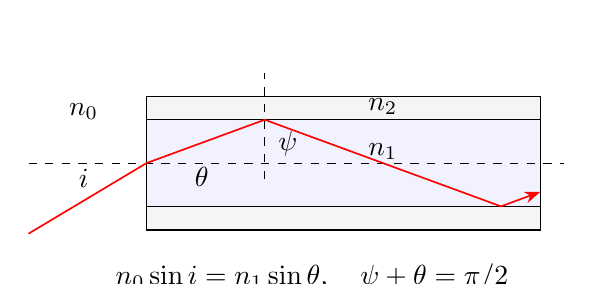
\begin{tikzpicture}[scale=1]
\draw[fill=gray!8] (0,-.85) rectangle(5,.85);
\draw[fill=blue!5] (0,-.55) rectangle(5,.55);
\draw[dashed] (-1.5,0)--(5.3,0);
\draw[arr,red] (-1.5,-.897)--(0,0)--(1.5,.55)--(4.5,-.55)--(5,-.3667);
\draw[dashed] (1.5,-.2)--(1.5,1.15);
\node at (-.8,-.2) {$i$};
\node at (.7,-.18) {$\theta$};
\node[right] at (1.55,.25) {$\psi$};
\node at (3,.15) {$n_1$}; \node at (3,.72) {$n_2$};
\node at (-.8,.65) {$n_0$};
\node at (2.1,-1.45) {$n_0\sin i=n_1\sin\theta,\quad\psi+\theta=\pi/2$};
\end{tikzpicture}
}
\ifdim\wd\diagrambox>.88\linewidth
\sbox{\diagrambox}{\resizebox{.88\linewidth}{!}{\usebox{\diagrambox}}}\fi
\ifdim\ht\diagrambox>.38\textheight
\resizebox{!}{.38\textheight}{\usebox{\diagrambox}}
\else\usebox{\diagrambox}\fi
\par\smallskip{\small 图6b　端面折射与芯包层全反射\par}\endgroup\end{minipage}\end{center}

（2）将光纤密绕\(N\)圈，首尾接于\(A\)，整个环路逆时针以\(\Omega\)转动。芯介质折射率为\(n_1\)，两束光真空波长为\(\lambda_0\)。求两束光传播\(N\)圈返回\(A\)的时间\(t_{\rm CCW},t_{\rm CW}\)、相位差，以及相位差与\(n_1\)的关系。

（3）旋转环形谐振腔半径为\(R\)，介质折射率\(n\)，\(R\Omega\ll c\)，腔和介质共同逆时针旋转。静止时模式满足\(2\pi R=m\lambda_{m0}\)，\(m\)为正整数、\(\lambda_{m0}\)为介质内波长。旋转时同一级次的CW、CCW共振模式有频率差\(\Delta f\)，求\(\Omega\)与\(\Delta f\)的关系。

\subsection{一、题型定位}\label{ux4e00ux9898ux578bux5b9aux4f4d-5}

第一问将端面折射与侧面全反射条件连接，得到光纤数值孔径。第二问是移动介质中光速的相对论合成，以及光与旋转分束器的追及问题。

第三问把相位累积转为共振频率，但必须保持频率、波长和模式编号在同一观察约定中。时间差不依赖折射率，并不意味着频率差也不依赖折射率：静态共振频率和腔的频率响应尺度均包含\(n\)。

本题参考解答的第三问采用另一套移动路径波长替代，给\(\Delta f\simeq m\Omega/\pi\)。下文保留参考解答的求法，并与共旋介质闭合腔的相位条件比较，说明两种处理为何不同。第一、二问的常用低速结果一致。

\subsection{二、知识点}\label{ux4e8cux77e5ux8bc6ux70b9-5}

\subsubsection{1.
端面折射与临界角}\label{ux7aefux9762ux6298ux5c04ux4e0eux4e34ux754cux89d2}

在平端面，法线沿光纤轴，折射光与轴线夹角记为\(\theta\)：

\[
n_0\sin i=n_1\sin\theta.
\]

在芯---包层侧面，入射角\(\psi\)相对于侧面法线，子午光线几何给

\[
\psi+\theta=\frac\pi2.
\]

全反射临界角

\[
\sin\psi_c=\frac{n_2}{n_1}.
\]

芯内传播应满足\(\psi\geq\psi_c\)的理想临界边界条件；为留有实际导光余量，应取严格大于。

\subsubsection{2.
移动介质中的相对论速度合成}\label{ux79fbux52a8ux4ecbux8d28ux4e2dux7684ux76f8ux5bf9ux8bbaux901fux5ea6ux5408ux6210}

介质局部静止系中沿纤维传播的光速为\(c/n\)。介质沿该局部切向以速度\(u\)运动，实验室沿同方向的光速

\[
v_+=\frac{c/n+u}{1+u/(nc)}.
\]

反方向光的有向速度为\((-c/n+u)/(1-u/(nc))\)；在\(u<c/n\)的通常范围内，其反向速率

\[
v_-=\frac{c/n-u}{1-u/(nc)}.
\]

低速展开为

\[
v_\pm\simeq\frac cn
\pm u\left(1-\frac1{n^2}\right).
\]

这是相对论速度合成给出的拖曳项，不能直接用\(c/n\pm u\)作实验室光速。

\subsubsection{3.
传播时间与分束器移动}\label{ux4f20ux64adux65f6ux95f4ux4e0eux5206ux675fux5668ux79fbux52a8}

令\(u=R\Omega>0\)，环路几何长度\(\ell=N2\pi R\)。CCW光追随分束器，需多走\(ut_{\rm CCW}\)；CW光迎向分束器，少走\(ut_{\rm CW}\)：

\[
v_+t_{\rm CCW}=\ell+ut_{\rm CCW},
\qquad
v_-t_{\rm CW}=\ell-ut_{\rm CW}.
\]

若只用\(\ell/v_\pm\)，会遗漏检测端的运动，得到错误时间差。

\subsubsection{4.
共振相位条件}\label{ux5171ux632fux76f8ux4f4dux6761ux4ef6}

静止腔某模式的一周相位必须为\(2\pi m\)：

\[
\frac{2\pi n f_0}{c}(2\pi R)=2\pi m,
\]

因此

\[
f_0=\frac{mc}{2\pi nR}
=\frac{c}{n\lambda_{m0}},
\qquad
\lambda_{\rm vac}=n\lambda_{m0}.
\]

介质内波长和真空波长不同。旋转后频率的变化必须由闭合相位条件求，不应把实验室移动路径长度配上未经变换的静止介质波长关系。

\subsection{三、物理图像}\label{ux4e09ux7269ux7406ux56feux50cf-5}

端面入射越斜，芯内光线相对轴线的角度越大，侧面入射角越小，越容易从芯泄漏到包层。数值孔径规定一个围绕轴线的接受锥。

\begin{center}
\begin{minipage}{\linewidth}
\centering\begingroup\sbox{\diagrambox}{\small
\begin{tikzpicture}[scale=1]
\draw[fill=blue!5] (0,-.6) rectangle(4,.6);
\draw[dashed] (-2.4,0)--(4.4,0);
\draw[blue,thick] (-2,-.9)--(0,0)--(-2,.9);
\draw[blue,dashed] (-2,-.9)--(-2,.9);
\draw[arr,red] (-2,-.45)--(0,0)--(2,.45);
\node at (-1.4,.45) {$i_{\max}$};
\node at (2,.95) {芯内导光};
\node at (1,-1.3) {$n_0|\sin i|\leq\sqrt{n_1^2-n_2^2}$};
\end{tikzpicture}
}
\ifdim\wd\diagrambox>.88\linewidth
\sbox{\diagrambox}{\resizebox{.88\linewidth}{!}{\usebox{\diagrambox}}}\fi
\ifdim\ht\diagrambox>.38\textheight
\resizebox{!}{.38\textheight}{\usebox{\diagrambox}}
\else\usebox{\diagrambox}\fi
\par\smallskip{\small 图6c　接受锥与临界导光边界\par}\endgroup\end{minipage}\end{center}

旋转环中，两束光不仅经历不同的实验室传播速率，还要与移动的\(A\)重合。相对分束器的两种传播速率在低速近似为

\[
v_+-u\simeq\frac cn-\frac{u}{n^2},
\qquad
v_-+u\simeq\frac cn+\frac{u}{n^2}.
\]

CCW相对分束器稍慢，返回时间较长。光速拖曳中的\((1-1/n^2)\)与分束器自身的\(u\)相减，形成关键的\(u/n^2\)修正。

\begin{center}
\begin{minipage}{\linewidth}
\centering\begingroup\sbox{\diagrambox}{\small
\begin{tikzpicture}[xscale=1.6,yscale=3]
\draw[arr] (-2,0)--(2.3,0) node[right] {$f-f_0$};
\draw[arr] (-2,0)--(-2,1.2) node[above] {共振响应};
\draw[thick,blue,domain=-1.9:1.9,samples=160] plot(\x,{1/(1+16*(\x+.5)^2)});
\draw[thick,red,domain=-1.9:1.9,samples=160] plot(\x,{1/(1+16*(\x-.5)^2)});
\node[blue] at (-.65,1.15) {CCW};
\node[red] at (.65,1.15) {CW};
\draw[<->] (-.5,1.42)--(.5,1.42) node[midway,above] {$\Delta f$};
\node at (0,-.4) {同级次相位闭合使两共振反向移动};
\end{tikzpicture}
}
\ifdim\wd\diagrambox>.88\linewidth
\sbox{\diagrambox}{\resizebox{.88\linewidth}{!}{\usebox{\diagrambox}}}\fi
\ifdim\ht\diagrambox>.38\textheight
\resizebox{!}{.38\textheight}{\usebox{\diagrambox}}
\else\usebox{\diagrambox}\fi
\par\smallskip{\small 图6d　固定光频下的相位与共振频率移动\par}\endgroup\end{minipage}\end{center}

固定外来光频时，旋转使一周相位在两方向上改变；若要求相位仍为同一个\(2\pi m\)，就要向相反方向调整两种模式的频率。这一调整量还要除以静态一周相位对频率的斜率。

\subsection{四、解题入口}\label{ux56dbux89e3ux9898ux5165ux53e3-5}

第一问用\(\sin\theta=\cos\psi\)把端面斯涅尔定律与侧面临界角连接。

第二问先由相对论合成得到\(v_\pm\)，再写追及式，最后相减。把两方向共用的\(n\)项和相反的\(u\)项分别保留，可以看出折射率如何抵消。

第三问以旋转坐标中的单周传播时间或单值相位条件求\(f_{\rm CW},f_{\rm CCW}\)。先算静态\(f_0\)，再求一阶转动修正；将同一级次\(m\)保持不变。

\subsection{五、解析}\label{ux4e94ux89e3ux6790-5}

\subsubsection{（1）芯包层的全反射条件}\label{ux82afux5305ux5c42ux7684ux5168ux53cdux5c04ux6761ux4ef6}

由侧面临界条件\(\psi\geq\psi_c\)，

\[
\theta\leq\frac\pi2-\psi_c.
\]

因此

\[
\sin\theta\leq\cos\psi_c
=\sqrt{1-\frac{n_2^2}{n_1^2}}.
\]

代入端面折射，

\[
n_0\sin i=n_1\sin\theta
\leq\sqrt{n_1^2-n_2^2}.
\]

故理想接受条件为

\[
\boxed{n_0|\sin i|\leq\sqrt{n_1^2-n_2^2}}.
\]

对\(0\leq i<\pi/2\)且右端除\(n_0\)不大于1时，

\[
\boxed{
i\leq i_{\max}
=\arcsin\frac{\sqrt{n_1^2-n_2^2}}{n_0}}.
\]

若\(\sqrt{n_1^2-n_2^2}/n_0>1\)，不能对大于1的实数取\(\arcsin\)；此几何模型下全部可入射角都满足该侧面临界约束。

定义数值孔径

\[
\mathrm{NA}=n_0\sin i_{\max}
=\sqrt{n_1^2-n_2^2}
\]

时，应理解通常接受角未饱和的情况。等号是临界边界，实际光束应留有角度余量。本题使用几何光学子午光线模型，不计算波导模式的截止细节。

\subsubsection{临界角与入射角不要混用}\label{ux4e34ux754cux89d2ux4e0eux5165ux5c04ux89d2ux4e0dux8981ux6df7ux7528}

侧面\(\psi\)相对于侧面法线，端面\(i\)相对于轴线法线，芯内\(\theta\)相对于轴线。三者有两个不同界面：

\[
n_0\sin i=n_1\sin\theta,\qquad
\psi=\frac\pi2-\theta.
\]

不能在端面直接要求\(i>\arcsin(n_2/n_1)\)；那会把不同法线的角度混在一起，并得出越斜越容易导光的相反结论。

\subsubsection{（2）两方向实验室传播速率}\label{ux4e24ux65b9ux5411ux5b9eux9a8cux5ba4ux4f20ux64adux901fux7387}

以下\(t_{\rm CCW},t_{\rm CW}\)取实验室坐标时间，使用题解的局部切向速度合成与固定几何长度模型。令\(u=R\Omega\)，

\[
v_+=\frac{c/n_1+u}{1+u/(n_1c)}
=\frac{c^2+n_1uc}{n_1c+u},
\]

\[
v_-=\frac{c/n_1-u}{1-u/(n_1c)}
=\frac{c^2-n_1uc}{n_1c-u}.
\]

两束光在介质静止系中的速率同为\(c/n_1\)，实验室速率不同。光纤约束让它们沿环路传播，方向随局部切线改变。

\subsubsection{从追及式求返回时间}\label{ux4eceux8ffdux53caux5f0fux6c42ux8fd4ux56deux65f6ux95f4}

由\(v_+t_{\rm CCW}=\ell+ut_{\rm CCW}\)，

\[
t_{\rm CCW}=\frac{\ell}{v_+-u}.
\]

分母化简为

\[
\begin{aligned}
v_+-u
&=\frac{c^2+n_1uc-u(n_1c+u)}{n_1c+u}\\
&=\frac{c^2-u^2}{n_1c+u}.
\end{aligned}
\]

因此

\[
\boxed{
t_{\rm CCW}
=\frac{N2\pi R(n_1c+R\Omega)}
{c^2-(R\Omega)^2}}.
\]

同理由\(v_-t_{\rm CW}=\ell-ut_{\rm CW}\)，

\[
v_-+u=\frac{c^2-u^2}{n_1c-u},
\]

所以

\[
\boxed{
t_{\rm CW}
=\frac{N2\pi R(n_1c-R\Omega)}
{c^2-(R\Omega)^2}}.
\]

这里共用的\(n_1c\)项决定平均传播时间，相反的\(R\Omega\)项决定方向差。

\subsubsection{时间差与折射率抵消}\label{ux65f6ux95f4ux5deeux4e0eux6298ux5c04ux7387ux62b5ux6d88}

相减得

\[
\boxed{
\Delta t=t_{\rm CCW}-t_{\rm CW}
=\frac{4\pi NR^2\Omega}
{c^2-(R\Omega)^2}}.
\]

常用低速\(R\Omega/c\ll1\)时，

\[
\boxed{\Delta t\simeq\frac{4N A\Omega}{c^2}},
\qquad A=\pi R^2.
\]

时间差与\(n_1\)无关，虽然各自传播时间约为\(N2\pi n_1R/c\)。如果把光速直接相加\(c/n_1\pm u\)，则相对分束器的两方向速率会被错误算成相同，甚至给出时间差零。

\subsubsection{相位差与光频定义}\label{ux76f8ux4f4dux5deeux4e0eux5149ux9891ux5b9aux4e49}

若\(\lambda_0\)按所用实验室光频\(f=c/\lambda_0\)定义，题解的相位差为

\[
\boxed{
\Delta\phi=2\pi f\Delta t
=\frac{8\pi^2NR^2\Omega c}
{\lambda_0[c^2-(R\Omega)^2]}}.
\]

低速结果

\[
\boxed{
\Delta\phi\simeq
\frac{8\pi N A\Omega}{\lambda_0c}}.
\]

对固定真空波长，它与\(n_1\)无关。旋转方向改变时\(\Omega\)变号，相位差也变号；交换CW、CCW的差值定义也使符号反转，但灵敏度大小不变。

若\(\lambda_0\)定义为分束器本地光源的真空波长，应以分束器固有时间差\(\Delta\tau=\Delta t\sqrt{1-u^2/c^2}\)配合本地光频。二者在一阶低速式完全一致，只在\(u^2/c^2\)及以上有差别。不能把不同参考系的精确时间与频率混用后声称所有高阶项也成立。

\subsubsection{N圈和面积的作用}\label{nux5708ux548cux9762ux79efux7684ux4f5cux7528}

在半径相同且绕向一致时，每一圈贡献同样的有向面积，因此时间差与相位差都乘\(N\)。在不等半径的多圈情况下，低速式中\(N\pi R^2\)应换成各圈有向面积之和。

增加光纤长度却不增加包围面积，不一定增加旋转相位灵敏度。这个结论由面积积分而非总光程本身决定。

\subsubsection{（3）共旋腔的静态模式}\label{ux5171ux65cbux8154ux7684ux9759ux6001ux6a21ux5f0f}

单圈长度\(\ell_1=2\pi R\)，静态一周时间

\[
t_0=\frac{n\ell_1}{c}.
\]

同一级次\(m\)的静态相位周期条件\(f_0t_0=m\)，所以

\[
f_0=\frac{mc}{n\ell_1}.
\]

由于题给\(\ell_1=m\lambda_{m0}\)，\(\lambda_{m0}\)是介质内波长，\(f_0=c/(n\lambda_{m0})\)。若把它当作真空波长，会少一个折射率因子。

\subsubsection{旋转一阶传播时间与闭合相位}\label{ux65cbux8f6cux4e00ux9636ux4f20ux64adux65f6ux95f4ux4e0eux95edux5408ux76f8ux4f4d}

从第二问取\(N=1,n_1=n\)并展开，

\[
t_{\rm CCW}=t_0+\frac{\ell_1u}{c^2}+O(u^2/c^2),
\]

\[
t_{\rm CW}=t_0-\frac{\ell_1u}{c^2}+O(u^2/c^2).
\]

在共旋坐标中，一个模式的场绕周必须恢复相位，因此同一\(m\)满足

\[
f_{\rm CCW}t_{\rm CCW}=m,\qquad
f_{\rm CW}t_{\rm CW}=m.
\]

保留一阶，倒数展开得

\[
f_{\rm CCW}
\simeq f_0\left(1-\frac{u}{nc}\right),
\qquad
f_{\rm CW}
\simeq f_0\left(1+\frac{u}{nc}\right).
\]

因此频差取正值\(f_{\rm CW}-f_{\rm CCW}\)：

\[
\begin{aligned}
\Delta f
&\simeq\frac{2f_0u}{nc}\\
&=\frac{2}{nc}\frac{mc}{2\pi nR}(R\Omega)\\
&=\boxed{\frac{m\Omega}{\pi n^2}}.
\end{aligned}
\]

故共旋、无色散闭合介质腔的相位自洽关系为

\[
\boxed{
\Omega\simeq\frac{\pi n^2}{m}\Delta f
=\frac{n^2\lambda_{m0}}{2R}\Delta f}.
\]

在这个低速精度内，共旋观察者的钟与实验室时间尺度差是二阶量，不改变上述一阶因子。

\subsubsection{从旋转坐标相速度再推导}\label{ux4eceux65cbux8f6cux5750ux6807ux76f8ux901fux5ea6ux518dux63a8ux5bfc}

实验室相速度一阶为\(c/n\pm u(1-1/n^2)\)。减去坐标本身的旋转，CCW相对于共旋角坐标的速度为

\[
\bar v_+=\frac cn-\frac{u}{n^2};
\]

CW反向速率为

\[
\bar v_-=\frac cn+\frac{u}{n^2}.
\]

闭合模式场形如\(e^{\pm im\varphi-i\omega_\pm t}\)，\(\varphi\)是共旋角坐标，空间单值性给波数大小\(m/R\)。因此

\[
\omega_{\rm CCW}=\frac mR\bar v_+,\qquad
\omega_{\rm CW}=\frac mR\bar v_-,
\]

得到\(\Delta\omega=2m\Omega/n^2\)，再次给\(\Delta f=m\Omega/(\pi n^2)\)。这条路线明确保持角波数和频率的同一坐标定义。

\subsubsection{固定光频与固定m的折射率依赖}\label{ux56faux5b9aux5149ux9891ux4e0eux56faux5b9amux7684ux6298ux5c04ux7387ux4f9dux8d56}

若使用真空波长\(\lambda_{\rm vac}=c/f_0\)，

\[
\boxed{
\Delta f\simeq
\frac{2R\Omega}{n\lambda_{\rm vac}}
=\frac{4A\Omega}{n\ell_1\lambda_{\rm vac}}}.
\]

固定\(f_0,R\)时，频差与\(1/n\)成正比；固定\(m,R\)时，因为\(f_0\)本身还与\(1/n\)成正比，频差与\(1/n^2\)成正比。两个结论描述不同的参数保持条件，并不冲突。

若介质有明显色散，静态相位对频率的导数还涉及群折射率，本题未给这类信息，以上采用\(n\)与频率无关的模型。

\par\noindent\begin{minipage}{\linewidth}
\subsubsection{参考解答的第三问约定}\label{ux53c2ux8003ux89e3ux7b54ux7684ux7b2cux4e09ux95eeux7ea6ux5b9a}

参考解答取两方向的实验室移动路径

\[
L_{\rm CW}=v_-t_{\rm CW},\qquad
L_{\rm CCW}=v_+t_{\rm CCW},
\]

再令\(L_\pm=m\lambda_\pm\)，并同时使用\(f_\pm=c/(n\lambda_\pm)\)，得到

\[
\Delta f_{\rm ref}
=\frac{m\Omega}{\pi}
\frac{c^2-u^2}{c^2-n^2u^2}
\simeq\frac{m\Omega}{\pi}.
\]

按该参考路径替代，答案为

\[
\boxed{\Omega_{\rm ref}\simeq\frac\pi m\Delta f}.
\]

然而移动介质中的实验室频率---波数关系已经因速度合成与多普勒变换改变，不再是静止介质的\(f=c/(n\lambda)\)。把移动路径和静止波长关系同时使用，不能与共旋腔场的单值相位条件等同。

因此备考时可识别参考采用的式子，物理建模时应明确区分它与前述相位闭合结果。\(n=1\)时两者一致；\(n\neq1\)时差异是一阶旋转灵敏度的\(n^2\)因子，不能归为二阶小量或数值舍入。

\subsubsection{时间差不等于频率差的直观核对}\label{ux65f6ux95f4ux5deeux4e0dux7b49ux4e8eux9891ux7387ux5deeux7684ux76f4ux89c2ux6838ux5bf9}

固定光频的相位差是\(\Delta\phi=2\pi f_0\Delta t\)。共振频率调整满足

\[
\delta\phi\simeq2\pi t_0\,\delta f.
\]

所以两方向频差近似

\[
\Delta f\simeq f_0\frac{\Delta t}{t_0}.
\]

\(\Delta t\)虽不含\(n\)，但\(f_0/t_0\propto1/n^2\)（固定\(m\)），因此不能直接从时间差的折射率抵消推出频差也抵消。这个检查只用相位对频率的导数，就能定位问题。

\end{minipage}\par
\clearpage

\section{第 7
题　双黑洞旋近的辐射与轨道演化（40分）}\label{ux7b2c-7-ux9898-ux53ccux9ed1ux6d1eux65cbux8fd1ux7684ux8f90ux5c04ux4e0eux8f68ux9053ux6f14ux531640ux5206}

双黑洞并合分为旋近、并合、衰荡三个阶段。旋近阶段，两黑洞绕系统质心在同一平面内作近似圆周运动，机械能损失转为引力波辐射能，间距\(L\)逐渐减小。

在旋近阶段忽略黑洞自转与大小，将它们视为质量\(M,m\)的质点。系统除引力波辐射外没有能量耗散；不考虑辐射反作用的详细形式，轨道关系用牛顿引力近似。

\begin{center}
\begin{minipage}{\linewidth}
\centering\begingroup\sbox{\diagrambox}{\small
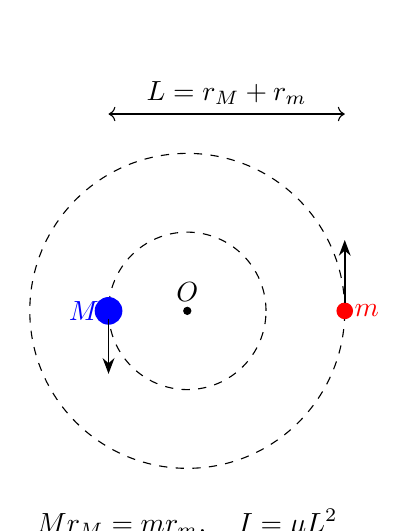
\begin{tikzpicture}[scale=1]
\draw[dashed] (0,0) circle(1); \draw[dashed] (0,0) circle(2);
\fill[blue] (-1,0) circle(5pt) node[left] {$M$};
\fill[red] (2,0) circle(3pt) node[right] {$m$};
\fill (0,0) circle(1.5pt) node[above] {$O$};
\draw[arr] (-1,-.1)--(-1,-.8); \draw[arr] (2,.1)--(2,.9);
\draw[<->] (-1,2.5)--(2,2.5) node[midway,above] {$L=r_M+r_m$};
\node at (0,-2.7) {$Mr_M=mr_m,\quad I=\mu L^2$};
\end{tikzpicture}
}
\ifdim\wd\diagrambox>.88\linewidth
\sbox{\diagrambox}{\resizebox{.88\linewidth}{!}{\usebox{\diagrambox}}}\fi
\ifdim\ht\diagrambox>.38\textheight
\resizebox{!}{.38\textheight}{\usebox{\diagrambox}}
\else\usebox{\diagrambox}\fi
\par\smallskip{\small 图7a　双质点绕共同质心旋近\par}\endgroup\end{minipage}\end{center}

（1）辐射功率与\(G\)正比，可与\(M,m,L\)、绕质心的转动惯量\(I\)、角速度\(\omega\)、辐射传播速度\(c\)有关。取描述转动体系的三个物理量，与\(G\)一起用量纲分析求功率形式，无量纲比例系数记为\(\alpha\)。

（2）已知\(t=0\)时两黑洞间距\(L_0\)，\(\alpha\)为已知常量。求两黑洞从\(t=0\)开始绕系统质心旋转360°所需时间。

（3）求当间距缩为\(L_0/2\)时，自初始时刻起旋转的度数。

\subsection{一、题型定位}\label{ux4e00ux9898ux578bux5b9aux4f4d-6}

本题用量纲分析建立辐射功率，再用近似圆轨道关系和能量守恒把辐射转成轨道参数演化。系统失去机械能，轨道能量变得更负，间距减小、角速度升高。

第二问不能以初始角速度固定不变算\(2\pi/\omega_0\)，因为旋转过程中轨道在缩小。应求角速度随时间的变化并积分角位移。

牛顿准圆旋近模型有适用区间。形式上间距可降到零，但真实黑洞会进入并合；若代数式要求越过这一模型端点，不能给出没有物理分支的``一整圈时间''。

\subsection{二、知识点}\label{ux4e8cux77e5ux8bc6ux70b9-6}

\subsubsection{1. 量纲选择}\label{ux91cfux7eb2ux9009ux62e9}

描述转动体系选择\(I,\omega,c\)。设

\[
P=\alpha G I^a\omega^bc^d.
\]

已知

\[
[G]=\mathrm{L^3M^{-1}T^{-2}},
\quad [I]=\mathrm{ML^2},
\quad[\omega]=\mathrm{T^{-1}},
\quad[c]=\mathrm{LT^{-1}}.
\]

功率量纲为\(\mathrm{ML^2T^{-3}}\)。这里\(\alpha\)承载量纲分析不能决定的纯数信息；题目后续假设它是给定常量。

\subsubsection{2.
质心与约化质量}\label{ux8d28ux5fc3ux4e0eux7ea6ux5316ux8d28ux91cf}

令总质量\(S=M+m\)，约化质量

\[
\mu=\frac{Mm}{M+m}.
\]

两质点到质心的距离\(r_M,r_m\)满足

\[
Mr_M=mr_m,\qquad r_M+r_m=L,
\]

故

\[
r_M=\frac mS L,\qquad r_m=\frac MS L.
\]

绕质心的总惯量

\[
I=Mr_M^2+mr_m^2=\mu L^2.
\]

\subsubsection{3. 圆轨道关系}\label{ux5706ux8f68ux9053ux5173ux7cfb}

两质点分别受同样大小的引力\(GMm/L^2\)。对较小质量\(m\)写

\[
\frac{GMm}{L^2}=m\omega^2r_m.
\]

代\(r_m=ML/S\)，得到

\[
\boxed{\omega^2=\frac{GS}{L^3}}.
\]

轨道总动能

\[
K=\frac12I\omega^2=\frac{GMm}{2L},
\]

引力势能\(U=-GMm/L\)，故总机械能

\[
\boxed{E=-\frac{GMm}{2L}}.
\]

\subsubsection{4.
辐射能量平衡}\label{ux8f90ux5c04ux80fdux91cfux5e73ux8861}

辐射功率\(P>0\)使系统机械能变化为

\[
\frac{dE}{dt}=-P.
\]

因为\(E(L)\)随\(L\)增大而增大，\(dE/dL=GMm/(2L^2)>0\)，所以失能必有\(\dot L<0\)。

\subsection{三、物理图像}\label{ux4e09ux7269ux7406ux56feux50cf-6}

两质点相对质心有相同角速度，但转动半径不同。较重质点靠近质心，较轻质点离质心较远，所有轨道关系可以由约化质量集中表示。

辐射使\(E\)降低，即变得更负。由\(\omega\propto L^{-3/2}\)，旋转越来越快；引力波频率随之升高，形成``啁啾''的频率增长。

\begin{center}
\begin{minipage}{\linewidth}
\centering\begingroup\sbox{\diagrambox}{\small
\begin{tikzpicture}[xscale=6,yscale=1]
\draw[arr] (0,0)--(1.12,0) node[right] {$t/t_c$};
\draw[arr] (0,0)--(0,4.6);
\draw[thick,blue,domain=0:.98,samples=150] plot(\x,{(1-\x)^.25});
\draw[thick,red,domain=0:.98,samples=150] plot(\x,{(1-\x)^(-.375)});
\draw[dashed] (.9375,0)--(.9375,2.828);
\node[below] at (.9375,0) {$15/16$};
\node[blue] at (.35,.45) {$L/L_0$};
\node[red] at (.62,2.6) {$\omega/\omega_0$};
\node at (.5,-.9) {近端点时近圆牛顿模型失效};
\end{tikzpicture}
}
\ifdim\wd\diagrambox>.88\linewidth
\sbox{\diagrambox}{\resizebox{.88\linewidth}{!}{\usebox{\diagrambox}}}\fi
\ifdim\ht\diagrambox>.38\textheight
\resizebox{!}{.38\textheight}{\usebox{\diagrambox}}
\else\usebox{\diagrambox}\fi
\par\smallskip{\small 图7b　间距与角速度的归一化演化\par}\endgroup\end{minipage}\end{center}

图中的横坐标使用形式上的演化时间尺度，越接近端点，间距下降越快、频率增长越快。靠近端点时慢变化近圆轨道与牛顿近似都会失效，应在实际适用范围内解释。

\subsection{四、解题入口}\label{ux56dbux89e3ux9898ux5165ux53e3-6}

先量纲求\(P\)，再代\(I=\mu L^2\)和\(\omega^2=GS/L^3\)，将功率化成单一\(L\)函数。对\(E(L)\)求导得到一阶\(\dot L\)方程。

从\(L(t)\)求\(\omega(t)\)，积分

\[
\Delta\theta(t)=\int_0^t\omega(s)\,ds.
\]

第二问令\(\Delta\theta=2\pi\)并筛选\(t\)；第三问先求\(L/L_0=1/2\)对应的参数，再算角位移，最后换成度。

\subsection{五、解析}\label{ux4e94ux89e3ux6790-6}

\subsubsection{（1）辐射功率的量纲}\label{ux8f90ux5c04ux529fux7387ux7684ux91cfux7eb2}

代入量纲，

\[
[G I^a\omega^bc^d]
=\mathrm{M^{a-1}L^{3+2a+d}T^{-2-b-d}}.
\]

与\(\mathrm{ML^2T^{-3}}\)比较，得到

\[
a-1=1,\qquad 3+2a+d=2,\qquad -2-b-d=-3.
\]

依次解出

\[
a=2,\qquad d=-5,\qquad b=6.
\]

因此

\[
\boxed{P=\frac{\alpha G I^2\omega^6}{c^5}}.
\]

量纲正确：

\[
\frac{(\mathrm{L^3M^{-1}T^{-2}})
(\mathrm{M^2L^4})(\mathrm{T^{-6}})}
{\mathrm{L^5T^{-5}}}
=\mathrm{ML^2T^{-3}}.
\]

这个分析不能单独确定\(\alpha\)的数值，也不能证明所有辐射体系都只有这三个参数；它依据题目指定的近圆双质点模型和选取的转动变量。

\subsubsection{将辐射功率写成间距函数}\label{ux5c06ux8f90ux5c04ux529fux7387ux5199ux6210ux95f4ux8dddux51fdux6570}

利用\(I=\mu L^2\)、\(\omega^6=G^3S^3/L^9\)，

\[
\begin{aligned}
P
&=\frac{\alpha G}{c^5}
\mu^2L^4\frac{G^3S^3}{L^9}\\
&=\frac{\alpha G^4\mu^2S^3}{c^5L^5}\\
&=\boxed{\frac{\alpha G^4M^2m^2S}{c^5L^5}}.
\end{aligned}
\]

功率随间距的五次倒数增长。虽然惯量随\(L^2\)降低，角速度六次方增长更强，使整体辐射增强。

\subsubsection{（2）间距的微分方程}\label{ux95f4ux8dddux7684ux5faeux5206ux65b9ux7a0b}

机械能\(E=-GMm/(2L)\)，所以

\[
\frac{dE}{dt}
=\frac{GMm}{2L^2}\dot L.
\]

令其等于\(-P\)，

\[
\frac{GMm}{2L^2}\dot L
=-\frac{\alpha G^4M^2m^2S}{c^5L^5}.
\]

定义正量

\[
\boxed{\mathcal A=\frac{2\alpha G^3MmS}{c^5}},
\]

量纲为\(\mathrm{L^4/T}\)。得到

\[
\boxed{\dot L=-\frac{\mathcal A}{L^3}}.
\]

对两边乘\(4L^3\)，

\[
\frac{d(L^4)}{dt}=-4\mathcal A.
\]

积分并用\(L(0)=L_0\)，

\[
\boxed{L(t)=[L_0^4-4\mathcal A t]^{1/4}}.
\]

选择正根，因为间距为正。形式解的时间范围\(0\leq t<t_c\)，其中

\[
\boxed{
t_c=\frac{L_0^4}{4\mathcal A}
=\frac{c^5L_0^4}{8\alpha G^3MmS}}.
\]

该\(t_c\)是本模型的形式端点，不是对真实黑洞并合时刻的完整预测。

\subsubsection{角速度随时间增加}\label{ux89d2ux901fux5ea6ux968fux65f6ux95f4ux589eux52a0}

初始角速度

\[
\omega_0=\sqrt{\frac{GS}{L_0^3}}.
\]

由圆轨道关系，

\[
\boxed{
\omega(t)=\omega_0
\left(1-\frac t{t_c}\right)^{-3/8}}.
\]

初始角速度随辐射而增大，指数\(-3/8\)来自\(L\propto(1-t/t_c)^{1/4}\)与\(\omega\propto L^{-3/2}\)的组合。

\subsubsection{角位移的积分}\label{ux89d2ux4f4dux79fbux7684ux79efux5206}

积分

\[
\Delta\theta(t)
=\omega_0\int_0^t
\left(1-\frac s{t_c}\right)^{-3/8}ds.
\]

令\(z=1-s/t_c\)，\(ds=-t_cdz\)，上下限从1到\(1-t/t_c\)。因此

\[
\begin{aligned}
\Delta\theta(t)
&=\omega_0t_c
\int_{1-t/t_c}^1z^{-3/8}dz\\
&=\frac85\omega_0t_c
\left[1-\left(1-\frac t{t_c}\right)^{5/8}\right].
\end{aligned}
\]

定义

\[
\boxed{
\Theta_c=\frac85\omega_0t_c
=\frac{c^5L_0^{5/2}}
{5\alpha G^{5/2}Mm\sqrt S}}.
\]

于是

\[
\boxed{
\Delta\theta(t)=\Theta_c
\left[1-\left(1-\frac t{t_c}\right)^{5/8}\right]}.
\]

\(\Theta_c\)是形式上从\(L_0\)到零间距的累计角位移。角速度虽然在端点发散，积分仍有限，因为指数\(3/8<1\)。

\subsubsection{一整圈时间的分支条件}\label{ux4e00ux6574ux5708ux65f6ux95f4ux7684ux5206ux652fux6761ux4ef6}

令\(\Delta\theta=2\pi\)，定义

\[
\chi=\frac{2\pi}{\Theta_c}
=\frac{10\pi\alpha G^{5/2}Mm\sqrt S}
{c^5L_0^{5/2}}.
\]

方程为

\[
\left(1-\frac{t_1}{t_c}\right)^{5/8}=1-\chi.
\]

左侧在物理分支非负。若希望整圈在正间距处完成，需

\[
\boxed{0<\chi<1}.
\]

此时

\[
\boxed{
t_1=t_c\left[1-(1-\chi)^{8/5}\right]}.
\]

用原参数展开，

\[
\boxed{
\begin{aligned}
t_1={}&\frac{c^5L_0^4}{8\alpha G^3Mm(M+m)}\\
&\times\left\{
1-\left[
1-\frac{10\pi\alpha G^{5/2}Mm\sqrt{M+m}}
{c^5L_0^{5/2}}
\right]^{8/5}
\right\}.
\end{aligned}}
\]

若\(\chi=1\)，形式整圈恰好在零间距端点完成，而端点不属于慢旋近有效区；若\(\chi>1\)，这个模型在端点前累计转角不足一圈。不能将负的\(1-\chi\)取分数幂并将其解释成另一条真实时间解。

\subsubsection{缓慢耗散的周期检查}\label{ux7f13ux6162ux8017ux6563ux7684ux5468ux671fux68c0ux67e5}

当\(\chi\ll1\)，二项展开

\[
1-(1-\chi)^{8/5}
=\frac85\chi-\frac{12}{25}\chi^2+O(\chi^3).
\]

利用\(t_c(8/5)\chi=2\pi/\omega_0\)，

\[
\boxed{
t_1=\frac{2\pi}{\omega_0}
\left[1-\frac3{10}\chi+O(\chi^2)\right]}.
\]

无耗散极限\(\alpha\to0\)时，\(\chi\to0\)、\(t_c\to\infty\)，乘积保持有限，恢复初始轨道周期。实际\(t_1\)略短于该周期，因为角速度在一圈内逐渐增大。

\subsubsection{（3）间距缩小一半的时间}\label{ux95f4ux8dddux7f29ux5c0fux4e00ux534aux7684ux65f6ux95f4}

令\(L=L_0/2\)，则

\[
\left(\frac L{L_0}\right)^4
=1-\frac t{t_c}=\frac1{16}.
\]

因此

\[
\boxed{
t_{1/2}=\frac{15}{16}t_c
=\frac{15c^5L_0^4}
{128\alpha G^3MmS}}.
\]

求得这段时间后，还需积分角速度并换算为度；时间结果也可用于核对中间计算。

\subsubsection{半间距对应的累计角位移}\label{ux534aux95f4ux8dddux5bf9ux5e94ux7684ux7d2fux8ba1ux89d2ux4f4dux79fb}

代\(1-t/t_c=1/16\)，

\[
\left(1-\frac{t_{1/2}}{t_c}\right)^{5/8}
=16^{-5/8}=2^{-5/2}=\frac{\sqrt2}{8}.
\]

所以弧度为

\[
\boxed{
\Delta\theta_{1/2}
=\Theta_c\left(1-\frac{\sqrt2}{8}\right)}.
\]

换成度数，

\[
\boxed{
\begin{aligned}
\Delta\theta_{1/2}^{(\deg)}
={}&\left(1-\frac{\sqrt2}{8}\right)
\frac{c^5L_0^{5/2}}
{5\alpha G^{5/2}Mm\sqrt{M+m}}\\
&\times\frac{180^\circ}{\pi}.
\end{aligned}}
\]

角位移不是将初始\(\omega_0\)乘\(t_{1/2}\)。这一段经历很大的频率变化：半间距时\(\omega/\omega_0=2^{3/2}=2\sqrt2\)。

\subsubsection{直接对间距积分的独立路线}\label{ux76f4ux63a5ux5bf9ux95f4ux8dddux79efux5206ux7684ux72ecux7acbux8defux7ebf}

由\(\dot L=-\mathcal A/L^3\)，

\[
dt=-\frac{L^3}{\mathcal A}\,dL.
\]

角位移微元

\[
d\theta=\omega\,dt
=-\frac{\sqrt{GS}}{\mathcal A}L^{3/2}\,dL.
\]

从\(L_0\)积分到\(L\)，

\[
\boxed{
\Delta\theta(L)
=\frac{2\sqrt{GS}}{5\mathcal A}
(L_0^{5/2}-L^{5/2})}.
\]

代\(L=L_0(1-t/t_c)^{1/4}\)恢复先前时间式，代\(L=L_0/2\)恢复半间距结果。这个积分将微分方程与角运动关系直接相接，提供不同消元路径。

\subsubsection{用角速度方程再检查}\label{ux7528ux89d2ux901fux5ea6ux65b9ux7a0bux518dux68c0ux67e5}

由\(\omega=\sqrt{GS}L^{-3/2}\)，

\[
\dot\omega=-\frac32\sqrt{GS}L^{-5/2}\dot L
=\frac32\mathcal A\sqrt{GS}L^{-11/2}.
\]

消去\(L\)，

\[
\boxed{
\dot\omega
=\frac{3\alpha G^{5/3}Mm}
{c^5S^{1/3}}\omega^{11/3}}.
\]

分离变量，

\[
\omega^{-11/3}d\omega
=\frac{3\alpha G^{5/3}Mm}{c^5S^{1/3}}dt,
\]

积分得

\[
\omega^{-8/3}
=\omega_0^{-8/3}
-\frac{8\alpha G^{5/3}Mm}{c^5S^{1/3}}t.
\]

它与\(\omega(t)=\omega_0(1-t/t_c)^{-3/8}\)一致，独立核对了幂次和系数。

\subsubsection{近圆与牛顿近似的适用条件}\label{ux8fd1ux5706ux4e0eux725bux987fux8fd1ux4f3cux7684ux9002ux7528ux6761ux4ef6}

径向变化相对一圈运动必须缓慢：

\[
\epsilon_{\rm ad}
=\frac{|\dot L|}{L\omega}
=\frac{\mathcal A}{\sqrt{GS}\,L^{5/2}}\ll1.
\]

牛顿轨道速度尺度\(\omega L=\sqrt{GS/L}\)也应明显小于\(c\)，即\(GS/(Lc^2)\ll1\)。随着\(L\)减小，两个条件都会变差。

因此形式解在\(t_c\)附近的发散主要提示模型失效。题目关注旋近阶段，不能把这条近似曲线当作真实并合或衰荡的完整解。

\clearpage

\section{第 8
题　电光调制与并联谐振驱动（40分）}\label{ux7b2c-8-ux9898-ux7535ux5149ux8c03ux5236ux4e0eux5e76ux8054ux8c10ux632fux9a71ux52a840ux5206}

电光调制将电信号转入光信号。以铌酸锂晶体为例，折射率随外电场变化，使光程改变。起偏器\(P_1\)与检偏器\(P_2\)相互正交，透光轴分别沿\(x_1,x_2\)。长度\(l\)、厚度\(d\)的晶体位于二者之间，电场沿光的传播方向\(x_3\)，大小\(E\)，晶体两端面加电压\(V\)。

\begin{center}
\begin{minipage}{\linewidth}
\centering\begingroup\sbox{\diagrambox}{\small
\begin{tikzpicture}[scale=.85]
\draw[arr,thick] (-1,0)--(9,0) node[right] {$x_3$光};
\draw[very thick] (0,-.8)--(0,.8);
\node[above] at (0,.85) {$P_1\parallel x_1$};
\draw[fill=blue!5,thick] (1,-.6) rectangle(5,.6);
\node at (3,.2) {电光晶体};
\node at (1,-.85) {$+$};\node at (5,-.85) {$-$};
\draw[<->] (1,1.3)--(5,1.3) node[midway,above] {$l$};
\draw[<->] (1,-1.3)--(5,-1.3) node[midway,below] {$V,\ E=V/l$};
\draw[very thick] (6,-.8)--(6,.8); \node[above] at (6,.85) {$1/4$波片};
\draw[very thick] (7.6,-.8)--(7.6,.8); \node[above] at (7.8,1.4) {$P_2\parallel x_2$};
\draw[arr] (3,-3.8)--(3,-2.8) node[above] {$x_1$};
\draw[arr] (3,-3.8)--(4,-3.8) node[right] {$x_2$};
\draw[arr,blue] (3,-3.8)--(2.3,-3.1) node[left] {$x'_1$};
\draw[arr,red] (3,-3.8)--(3.7,-3.1) node[right] {$x'_2$};
\end{tikzpicture}
}
\ifdim\wd\diagrambox>.88\linewidth
\sbox{\diagrambox}{\resizebox{.88\linewidth}{!}{\usebox{\diagrambox}}}\fi
\ifdim\ht\diagrambox>.38\textheight
\resizebox{!}{.38\textheight}{\usebox{\diagrambox}}
\else\usebox{\diagrambox}\fi
\par\smallskip{\small 图8a　偏振分解、晶体与四分之一波片\par}\endgroup\end{minipage}\end{center}

真空波长\(\lambda_0\)的光经\(P_1\)后沿\(x_3\)入射，分解为晶体快轴\(x'_1\)与慢轴\(x'_2\)上的正交分量。两主轴与\(x_1,x_2\)均呈45°，折射率为

\[
n_{x'_1}=n_0-\frac12n_0^3\gamma E,\qquad
n_{x'_2}=n_0+\frac12n_0^3\gamma E.
\]

\(\gamma\)为材料常量。光出晶体后经过1/4波片，再由\(P_2\)检出。采用题图主轴对齐、波片给慢快分量额外\(+\pi/2\)延迟的约定。

（1）入射到晶体左端面的两分量电场为\(E_{x'_1}=E_0\cos\omega t\)、\(E_{x'_2}=E_0\cos\omega t\)。求经过晶体的相位变化和光强变化；出射两分量相位差为\(\pi\)时称晶体为1/2波片，求半波电压\(V_\pi\)。

（2）调制电压\(V=V_m\sin\omega_mt\)，\(V_m\ll V_\pi\)。先求不经过1/4波片、直接经\(P_2\)后的光强透过率与\(V\)的关系；再求经过1/4波片与\(P_2\)的透过率，指出1/4波片的作用。

（3）晶体的等效电路为并联电阻\(R\)和电容\(C\)，电源串联电阻\(R_m\)，\(R\gg R_m\)。开关断开时，证明当\(\omega_m\gg(R_mC)^{-1}\)，晶体实际电压\(|V_c|\ll|V|\)。

\begin{center}
\begin{minipage}{\linewidth}
\centering\begingroup\sbox{\diagrambox}{\small
\begin{tikzpicture}[scale=.9]
\draw[thick] (0,0)--(0,.6); \draw[thick] (0,1) circle(.4); \node at (0,1) {$V$};
\draw[thick] (0,1.4)--(0,2)--(.8,2);
\draw[thick] (.8,1.8) rectangle(1.8,2.2); \node[above] at (1.3,2.3) {$R_m$};
\draw[thick] (1.8,2)--(5.1,2);
\draw[thick] (3,2)--(3,1.4); \draw[thick] (2.8,.6) rectangle(3.2,1.4);
\node[left] at (2.8,1) {$R$};\draw[thick] (3,.6)--(3,0);
\draw[thick] (4.4,2)--(4.4,1.15); \draw[thick] (4.1,1.15)--(4.7,1.15);
\draw[thick] (4.1,.95)--(4.7,.95); \draw[thick] (4.4,.95)--(4.4,0);
\node[right] at (4.65,1) {$C$};
\draw (5.1,2) circle(1.5pt); \draw (5.8,2) circle(1.5pt);
\draw[thick] (5.1,2)--(5.7,2.35); \node at (5.4,2.7) {$S$};
\draw[thick] (5.8,2)--(7.7,2);
\draw[thick] (6.2,2)--(6.2,1.6);
\draw[thick,decorate,decoration={coil,aspect=.3,segment length=4pt,amplitude=3pt}] (6.2,1.6)--(6.2,.5);
\draw[thick] (6.2,.5)--(6.2,0); \node[right] at (6.5,1) {$L$};
\draw[thick] (7.7,2)--(7.7,1.4); \draw[thick] (7.5,.6) rectangle(7.9,1.4);
\node[right] at (7.9,1) {$R_L$}; \draw[thick] (7.7,.6)--(7.7,0)--(0,0);
\node at (4,-.8) {闭合$S$接入并联$L,R_L$};
\end{tikzpicture}
}
\ifdim\wd\diagrambox>.88\linewidth
\sbox{\diagrambox}{\resizebox{.88\linewidth}{!}{\usebox{\diagrambox}}}\fi
\ifdim\ht\diagrambox>.38\textheight
\resizebox{!}{.38\textheight}{\usebox{\diagrambox}}
\else\usebox{\diagrambox}\fi
\par\smallskip{\small 图8b　电源与晶体并联谐振补偿\par}\endgroup\end{minipage}\end{center}

（4）为提高调制效率，闭合开关，加入与晶体并联的谐振回路，电感为\(L\)、负载电阻为\(R_L\)。试证明\(|V_c|\simeq|V|\)。

\subsection{一、题型定位}\label{ux4e00ux9898ux578bux5b9aux4f4d-7}

前两问是偏振分解与电压控制的相位延迟，后两问是高频电源如何把电压送到电容性晶体。光学响应和电路分压共同决定真实调制效率。

理想晶体改变两正交分量的相位而不吸收能量；检偏器将相位差转成光强变化。正交检偏器在零相位差附近的透过率是二次小量，不能忠实保留弱电压信号的正负；四分之一波片将工作点移到最大斜率附近。

并联电感的作用是抵消电容的电纳。电感必须调谐到指定频率，且剩余并联电阻足够大，才能避免电源串联电阻把电压分走。

\subsection{二、知识点}\label{ux4e8cux77e5ux8bc6ux70b9-7}

\subsubsection{1.
相位延迟与纵向电场}\label{ux76f8ux4f4dux5ef6ux8fdfux4e0eux7eb5ux5411ux7535ux573a}

真空波长\(\lambda_0\)、介质折射率\(n_j\)、传播长度\(l\)的相位延迟为

\[
\phi_j=\frac{2\pi}{\lambda_0}n_jl.
\]

题面给电场沿传播\(x_3\)且加在两端面，因此使用纵向几何

\[
E=\frac Vl.
\]

厚度\(d\)不进入这一纵向电场表达式。若另改为厚度两侧加横向电场，才应使用\(E=V/d\)，半波电压也随\(d/l\)改变。

\subsubsection{2.
相干分量与光强}\label{ux76f8ux5e72ux5206ux91cfux4e0eux5149ux5f3a}

两个正交偏振分量可以各有相位，但未经分析器时总平均光强是两分量的平均强度之和，没有相互干涉项。

用复振幅\(a_1,a_2\)表示，并把平均光强比例常量记为\(K_o\)：

\[
I=K_o(|a_1|^2+|a_2|^2).
\]

检偏器将两个分量投影到同一个轴，投影后的复振幅才需先相加再求模平方，产生与相位差有关的干涉。

\subsubsection{3.
偏振主轴与投影符号}\label{ux504fux632fux4e3bux8f74ux4e0eux6295ux5f71ux7b26ux53f7}

选择

\[
\hat{\mathbf x}'_1=
\frac{\hat{\mathbf x}_1-\hat{\mathbf x}_2}{\sqrt2},
\qquad
\hat{\mathbf x}'_2=
\frac{\hat{\mathbf x}_1+\hat{\mathbf x}_2}{\sqrt2}.
\]

于是输入\(x_1\)方向是两主轴的等振幅和，输出\(x_2\)方向是两主轴的差：

\[
\hat{\mathbf x}_1=\frac{\hat{\mathbf x}'_1+\hat{\mathbf x}'_2}{\sqrt2},
\quad
\hat{\mathbf x}_2=\frac{-\hat{\mathbf x}'_1+\hat{\mathbf x}'_2}{\sqrt2}.
\]

检偏振幅中的负号是正交轴几何决定的，不是为了凑成某个三角函数。

\subsubsection{4. 高频相量}\label{ux9ad8ux9891ux76f8ux91cf}

采用\(e^{i\omega_mt}\)约定，

\[
Z_C=\frac1{i\omega_mC},\qquad Z_L=i\omega_mL.
\]

并联用导纳相加，串联用阻抗相加。晶体电压由串联\(R_m\)与整个并联网络分压：

\[
\frac{\widetilde V_c}{\widetilde V}
=\frac Z{R_m+Z}
=\frac1{1+R_mY}.
\]

\subsection{三、物理图像}\label{ux4e09ux7269ux7406ux56feux50cf-7}

输入\(x_1\)线偏振在两个45°主轴上有相等振幅。晶体令它们相位错开，形成一般椭圆偏振；无损情况下总光强不变。正交检偏器把两个主轴上的场带符号地投到\(x_2\)，相位差零时完全相消。

\begin{center}
\begin{minipage}{\linewidth}
\centering\begingroup\sbox{\diagrambox}{\small
\begin{tikzpicture}[xscale=5,yscale=3]
\draw[arr] (-.72,0)--(.82,0) node[right] {$V/V_\pi$};
\draw[arr] (0,0)--(0,1.2) node[above] {$\mathcal T$};
\draw[thick,blue,domain=-.7:.7,samples=120] plot(\x,{sin(90*\x)^2});
\draw[thick,red,domain=-.7:.7,samples=120] plot(\x,{(1+sin(180*\x))/2});
\draw[dashed,domain=-.25:.25] plot(\x,{.5+pi*\x/2});
\node[blue] at (-.42,1.3) {无波片};
\node[red] at (.42,1.3) {加$1/4$波片};
\node at (0,-.42) {固定$\pi/2$偏置使零电压处斜率非零};
\end{tikzpicture}
}
\ifdim\wd\diagrambox>.88\linewidth
\sbox{\diagrambox}{\resizebox{.88\linewidth}{!}{\usebox{\diagrambox}}}\fi
\ifdim\ht\diagrambox>.38\textheight
\resizebox{!}{.38\textheight}{\usebox{\diagrambox}}
\else\usebox{\diagrambox}\fi
\par\smallskip{\small 图8c　检偏透过率与电压偏置\par}\endgroup\end{minipage}\end{center}

不加波片时，\(V=0\)附近曲线是谷底，斜率零，正负电压产生相同光强。增加固定\(\pi/2\)延迟后，零调制附近位于透过率约1/2的最大斜率点，正负电压对应光强的上下变化。

高频下晶体电容阻抗很小，电流大，电源内阻上分走大部分电压。调谐电感后，电容和电感的无功电流在并联网络内相消，电源只需承担损耗电流。

\begin{center}
\begin{minipage}{\linewidth}
\centering\begingroup\sbox{\diagrambox}{\small
\begin{tikzpicture}[xscale=3,yscale=3]
\draw[arr] (.15,0)--(2.2,0) node[right] {$\omega/\omega_0$};
\draw[arr] (.15,0)--(.15,1.15) node[above] {$|V_c/V|$};
\draw[thick,blue,domain=.2:2,samples=150] plot(\x,{1/sqrt(1+25*\x*\x)});
\draw[thick,red,domain=.2:2,samples=250] plot(\x,{1/sqrt(1.01^2+25*(\x-1/\x)^2)});
\draw[dashed] (1,0)--(1,1); \node[below] at (1,0) {$1$};
\node[blue] at (.62,1.25) {无补偿};
\node[red] at (1.5,1.25) {谐振补偿};
\node at (1.2,-.42) {峰值受损耗限制，恢复只在调谐频带内};
\end{tikzpicture}
}
\ifdim\wd\diagrambox>.88\linewidth
\sbox{\diagrambox}{\resizebox{.88\linewidth}{!}{\usebox{\diagrambox}}}\fi
\ifdim\ht\diagrambox>.38\textheight
\resizebox{!}{.38\textheight}{\usebox{\diagrambox}}
\else\usebox{\diagrambox}\fi
\par\smallskip{\small 图8d　有无谐振补偿的电压响应\par}\endgroup\end{minipage}\end{center}

谐振补偿使一个选定频率附近的电压恢复，但不是宽带消除全部电容影响。负载和损耗决定峰值，调谐决定电纳是否相消。

\subsection{四、解题入口}\label{ux56dbux89e3ux9898ux5165ux53e3-7}

光学先求\(\delta=\phi_2-\phi_1\)，再用\(x_2\)投影求透过率。半波电压由\(\delta=\pi\)求，不由光强本身直接猜。

弱信号\(V_m\ll V_\pi\)意味着\(\delta_m=\pi V_m/V_\pi\ll1\)。先写精确三角函数响应，再展开；可以清楚区分二次响应和一阶线性响应。

电路先写导纳\(Y\)，再计算\(H=\widetilde V_c/\widetilde V\)。闭合开关后，谐振需要虚部为零，电压接近电源还需要实部远小于\(1/R_m\)，两个条件必须同时满足。

\subsection{五、解析}\label{ux4e94ux89e3ux6790-7}

\subsubsection{（1）经过晶体的两种相位}\label{ux7ecfux8fc7ux6676ux4f53ux7684ux4e24ux79cdux76f8ux4f4d}

由题给折射率，

\[
\phi_1=\frac{2\pi l}{\lambda_0}
\left(n_0-\frac12n_0^3\gamma E\right),
\]

\[
\phi_2=\frac{2\pi l}{\lambda_0}
\left(n_0+\frac12n_0^3\gamma E\right).
\]

相位差

\[
\begin{aligned}
\delta=\phi_2-\phi_1
&=\frac{2\pi l}{\lambda_0}n_0^3\gamma E\\
&=\boxed{\frac{2\pi n_0^3\gamma}{\lambda_0}V}.
\end{aligned}
\]

公共相位\((\phi_1+\phi_2)/2=2\pi n_0l/\lambda_0\)不会影响检偏后的强度，只影响整个场的共同相位。

取题给正向电压使\(\gamma E>0\)的主轴标号。若材料\(\gamma\)符号相反，可交换快慢轴或反转电压方向，半波电压大小使用\(|\gamma|\)。

\subsubsection{晶体本身的光强变化}\label{ux6676ux4f53ux672cux8eabux7684ux5149ux5f3aux53d8ux5316}

入射两个分量振幅均为\(E_0\)，所以

\[
I_{\rm in}=2K_oE_0^2.
\]

在忽略吸收及界面反射的理想相位延迟模型中，晶体只乘上相位因子，

\[
(a_1,a_2)
=(E_0e^{-i\phi_1},E_0e^{-i\phi_2}).
\]

故

\[
I_{\rm crystal}
=K_o(E_0^2+E_0^2)
=\boxed{I_{\rm in}}.
\]

相位差改变偏振态，不直接改变未经检偏的总光强。后续检偏器将部分偏振分量滤掉，才产生光强调制。

\subsubsection{半波电压}\label{ux534aux6ce2ux7535ux538b}

出射相位差\(\pi\)时，

\[
\frac{2\pi n_0^3\gamma}{\lambda_0}V_\pi=\pi.
\]

因此按正标号约定

\[
\boxed{V_\pi=\frac{\lambda_0}{2n_0^3\gamma}},
\qquad
\boxed{\delta=\pi\frac V{V_\pi}}.
\]

若求电压大小，\(|V_\pi|=\lambda_0/(2n_0^3|\gamma|)\)。纵向几何中\(l\)抵消：更长晶体增加光程相位积累，却使同一电压对应电场更小，两者正好抵消。

\(\gamma\)的量纲为m/V，故\(\lambda_0/\gamma\)为电压，量纲成立。不能因题面出现\(d\)就强行在纵向公式中加入\(d\)。

\subsubsection{（2）不加四分之一波片}\label{ux4e0dux52a0ux56dbux5206ux4e4bux4e00ux6ce2ux7247}

经\(x_2\)检偏后的复振幅

\[
a_{\rm out}
=\frac{E_0}{\sqrt2}
\left(-e^{-i\phi_1}+e^{-i\phi_2}\right).
\]

提取公共相位，

\[
|a_{\rm out}|^2
=\frac{E_0^2}{2}|e^{-i\delta}-1|^2.
\]

由于

\[
|e^{-i\delta}-1|^2=2-2\cos\delta
=4\sin^2(\delta/2),
\]

输出强度

\[
I_{\rm out}=2K_oE_0^2\sin^2(\delta/2).
\]

透过率

\[
\boxed{
\mathcal T_0=\frac{I_{\rm out}}{I_{\rm in}}
=\sin^2\left(\frac{\pi V}{2V_\pi}\right)}.
\]

当\(V=0\)，两分量相位相同，输入仍是\(x_1\)线偏振，正交\(x_2\)检偏器完全挡光；当\(V=V_\pi\)，半波延迟将线偏振转到\(x_2\)，理想透过率为1。

\subsubsection{弱交流信号的二次失真}\label{ux5f31ux4ea4ux6d41ux4fe1ux53f7ux7684ux4e8cux6b21ux5931ux771f}

令\(a=\pi V_m/V_\pi\ll1\)，电压\(V=V_m\sin\omega_mt\)，则

\[
\mathcal T_0(t)
=\sin^2\left(\frac a2\sin\omega_mt\right)
\simeq\frac{a^2}{4}\sin^2\omega_mt.
\]

因此

\[
\boxed{
\mathcal T_0(t)\simeq
\frac{a^2}{8}[1-\cos(2\omega_mt)]}.
\]

弱信号中的一次频率\(\omega_m\)被变成直流项和二倍频项，电压正负被抹掉。这是工作点处斜率为零导致的非线性，不是光频率本身被改成两倍。

\subsubsection{加入四分之一波片}\label{ux52a0ux5165ux56dbux5206ux4e4bux4e00ux6ce2ux7247}

主轴与晶体相同的1/4波片为两分量增加固定相位差\(\delta_q=+\pi/2\)。总延迟\(\delta+\pi/2\)，检偏透过率

\[
\boxed{
\mathcal T_q
=\sin^2\left(\frac{\delta}{2}+\frac\pi4\right)
=\frac12(1+\sin\delta)}.
\]

弱电压展开，

\[
\boxed{
\mathcal T_q\simeq
\frac12+\frac{\pi}{2V_\pi}V}.
\]

对于正弦电压，

\[
\boxed{
\mathcal T_q(t)\simeq
\frac12+\frac{\pi V_m}{2V_\pi}\sin\omega_mt}.
\]

透过率有1/2的直流光背景，交流增量与电压同频、同号。波片使零电压工作点位于透过率曲线最大斜率处，完成弱信号的一阶线性化。

若波片慢快轴互换，\(\delta_q=-\pi/2\)，得到\(\mathcal T_q=(1-\sin\delta)/2\)，调制斜率反号，线性化能力相同。波片若任意转轴而非与晶体主轴匹配，则不能只简单将\(\pi/2\)加到原延迟上。

\subsubsection{线性化的局部范围}\label{ux7ebfux6027ux5316ux7684ux5c40ux90e8ux8303ux56f4}

精确响应仍为正弦，不是任意电压下的直线：

\[
\mathcal T_q
=\frac12+\frac{\delta}{2}
-\frac{\delta^3}{12}+O(\delta^5).
\]

相对于一次调制幅度，非线性修正随\(\delta_m^2\)增长。原题\(V_m\ll V_\pi\)保证局部近似有效。若一次直线近似预测\(\mathcal T<0\)或大于1，就已超出适用范围。

\subsubsection{用Jones矩阵核对偏振}\label{ux7528jonesux77e9ux9635ux6838ux5bf9ux504fux632f}

在主轴基中，晶体与波片的无损相位矩阵为

\[
J=\begin{pmatrix}
e^{-i\phi_1}&0\\
0&e^{-i(\phi_2+\delta_q)}
\end{pmatrix}.
\]

输入归一化向量为\((1,1)^T/\sqrt2\)，检偏轴投影为\((-1,1)/\sqrt2\)。输出相对振幅

\[
\frac12\left[-e^{-i\phi_1}
+e^{-i(\phi_2+\delta_q)}\right].
\]

模平方为\(\sin^2[(\delta+\delta_q)/2]\)，同时恢复无波片和四分之一波片结果。矩阵满足\(J^\dagger J=1\)，解释了晶体与理想波片本身保持光强。

\subsubsection{（3）开关断开时的晶体阻抗}\label{ux5f00ux5173ux65adux5f00ux65f6ux7684ux6676ux4f53ux963bux6297}

晶体\(R,C\)并联，

\[
Y_c=\frac1R+i\omega_mC,\qquad
Z_c=\frac1{1/R+i\omega_mC}.
\]

与电源串联电阻分压，

\[
\boxed{
H_0(\omega_m)=\frac{\widetilde V_c}{\widetilde V}
=\frac1{1+R_m/R+i\omega_mR_mC}}.
\]

幅值为

\[
\boxed{
|H_0|
=\frac1{\sqrt{(1+R_m/R)^2+(\omega_mR_mC)^2}}}.
\]

用\(R\gg R_m\)，

\[
|H_0|\simeq
\frac1{\sqrt{1+(\omega_mR_mC)^2}}.
\]

当\(\omega_mR_mC\gg1\)，

\[
\boxed{
\frac{|V_c|}{|V|}
\simeq\frac1{\omega_mR_mC}\ll1}.
\]

电压几乎落在串联\(R_m\)上。相位为

\[
\arg H_0=-\arctan\frac{\omega_mR_mC}{1+R_m/R},
\]

高频时晶体电压近似滞后电源90°。调制除了幅度小，也具有电路相位延迟。

\subsubsection{晶体的真实光学调制幅度}\label{ux6676ux4f53ux7684ux771fux5b9eux5149ux5b66ux8c03ux5236ux5e45ux5ea6}

光学公式中的\(V\)应是晶体实际电压\(V_c\)，而非未经分压的电源电压。若输入电源幅值为\(V_m\)，实际一次调制幅度

\[
\Delta\mathcal T_m
\simeq\frac{\pi}{2V_\pi}|H_0(\omega_m)|V_m.
\]

高频衰减直接抑制光强调制。只检查材料半波电压，却忽略电源与电容分压，会高估真实转换效率。

\subsubsection{（4）闭合开关后的总导纳}\label{ux95edux5408ux5f00ux5173ux540eux7684ux603bux5bfcux7eb3}

加入理想电感\(L\)与负载电阻\(R_L\)后，整个并联网络导纳

\[
\boxed{
Y=\frac1R+\frac1{R_L}
+i\left(\omega_mC-\frac1{\omega_mL}\right)}.
\]

令

\[
G_e=\frac1R+\frac1{R_L},\qquad
B_e=\omega_mC-\frac1{\omega_mL},
\]

则

\[
\boxed{
H(\omega_m)=
\frac1{1+R_mG_e+iR_mB_e}}.
\]

因此

\[
\boxed{
|H|=
\frac1{\sqrt{(1+R_mG_e)^2+(R_mB_e)^2}}}.
\]

这条式子保留了晶体漏电损耗和负载损耗，没有在开始就将\(R\)略去。

\subsubsection{并联谐振的调谐条件}\label{ux5e76ux8054ux8c10ux632fux7684ux8c03ux8c10ux6761ux4ef6}

使电感与电容电纳相消，要求

\[
\boxed{\omega_mC-\frac1{\omega_mL}=0},
\quad
\boxed{L=\frac1{\omega_m^2C}}.
\]

此时网络阻抗纯实，

\[
Z_{\rm res}=\frac1{G_e}
=R_e,\qquad
R_e=\left(\frac1R+\frac1{R_L}\right)^{-1}.
\]

晶体电压比例为

\[
\boxed{
H_{\rm res}=\frac{R_e}{R_m+R_e}
=\frac1{1+R_m/R+R_m/R_L}}.
\]

因此\(|V_c|\simeq|V|\)还需要

\[
\boxed{R_e\gg R_m}.
\]

题给\(R\gg R_m\)只保证晶体本身漏电较小，还需负载\(R_L\gg R_m\)。只添加任意电感或任意低阻负载，不能保证电压恢复。

\subsubsection{谐振为何减少电源分压}\label{ux8c10ux632fux4e3aux4f55ux51cfux5c11ux7535ux6e90ux5206ux538b}

在谐振频率，电容和电感各有无功电流

\[
\widetilde I_C=i\omega_mC\widetilde V_c,\qquad
\widetilde I_L=-\frac{i}{\omega_mL}\widetilde V_c.
\]

二者相消，电源只供\(G_e\widetilde V_c\)的同相损耗电流。串联电阻压降因而减小，晶体电压接近电源。

这不意味着支路电流都小，也不意味着网络创造能量。理想电感与电容不断交换储能，电源负责各电阻的平均损耗。真实电感若有额外损耗，需要把它也加入导纳实部。

\subsubsection{偏离谐振的频率响应}\label{ux504fux79bbux8c10ux632fux7684ux9891ux7387ux54cdux5e94}

设\(\omega_0=1/\sqrt{LC}\)，附近\(\omega=\omega_0+\Delta\omega\)且\(|\Delta\omega|\ll\omega_0\)。电纳展开

\[
B_e(\omega)\simeq2C\Delta\omega.
\]

所以

\[
|H(\omega)|
\simeq
\frac1{\sqrt{a_e^2+(2R_mC\Delta\omega)^2}},
\qquad a_e=1+R_mG_e.
\]

半功率点满足\(|H|^2=|H_{\rm res}|^2/2\)，因此

\[
|\Delta\omega|=\frac{a_e}{2R_mC}.
\]

峰越尖，偏离设计频率时恢复效果越差。题目第四问是在特定调制频率调谐，不是对任意输入频谱都给相同增益。

\end{document}
